\chapter{Results and Discussions} \label{chap:results}

%\section{Results and discussions}
\section{Results}
%Something to remember about figures
%\begin{itemize}
%    \item All the plots should be vector images in pdf format
%    \item Use raster images in jpg or png format only as a last resort
%    \item Remove white space from the figrues (do not clip/crop using latex setup)
%    \item Make sure that the fonts are readable. Make the text as big as possible but without making them appear ugly.
%    \item Make all the figure caption self-descriptive. Highlight the things you want to emphasize in the figures.
%    \item Avoid using figure titles in when you create the figures. It is always better to have sub-caption written in latex.
%    \item You can use draw.io tool for creating figures and then export as pdf. 
%    \item For plots you can use matplotlib
%\end{itemize}

%Just don't present the results, discuss them. If things have worked explain why they worked and if not then the probably reasons. 

\subsection{Learning Dynamical Systems with Physics Informed Neural Networks}

\subsubsection{Linear ODE}

Training both a standard neural network and a PINN with the same number of parameters in the networks, and using them to plot their output trajectories are visualized in Figure \ref{fig:msd}. Both models are able to closely follow the true trajectory at the beginning, as it is a relatively simple system and does not require that much data. However, after $t > 0.4$ seconds the neural network output is diverging from the true output as it was not trained on any data past this, and is therefore not generalizing outside its training set. This can also be interpreted as overfitting on the training points. This is normal behavior from a standard neural network and was to be expected. One possible solution is to add more data, but in many real life cases this is not feasible.

\begin{figure}[H]
    \centering
    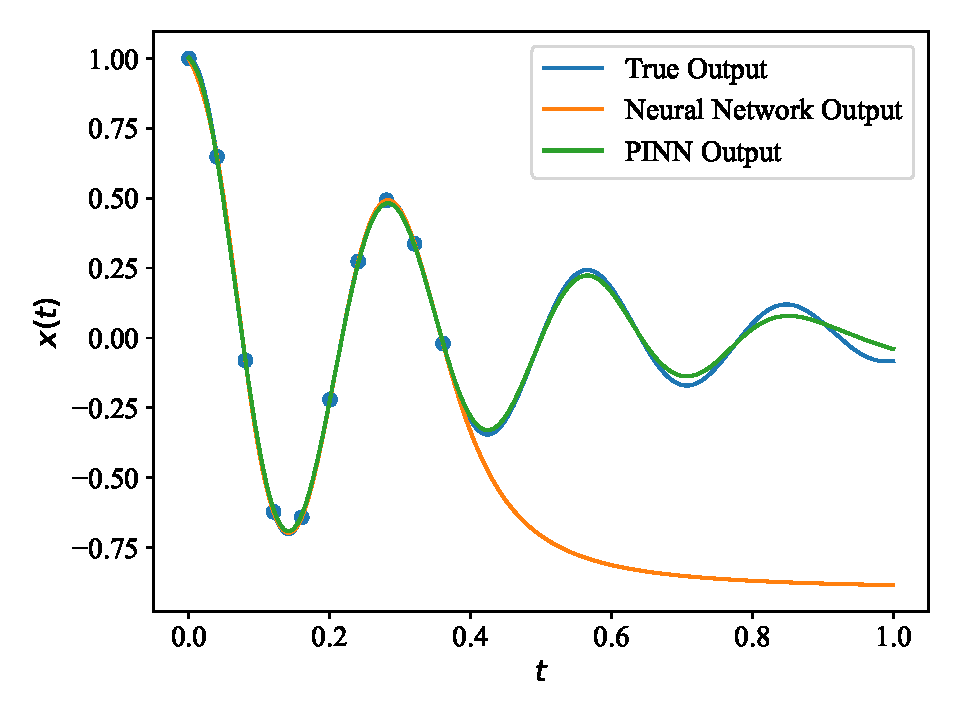
\includegraphics[width=1.0\linewidth]{Figures/InitialExperiments/msd.pdf}
    \caption{Output trajectories from a standard neural network and a PINN trained on a mass spring damper system. Datapoints are highlighted as blue dots.}
    \label{fig:msd}
\end{figure}

Adding a physics informed regularizer on the PINN results in much better generalization and follows the true system for much longer. Although the PINN is still not perfect towards the end, which is a consequence of the collocation points used during training. PINNs will not generalize further than their collocation points were sampled from, but as the collocation points can be generated at will when training it is necessary to first determine how long the PINN should stay accurate before training.

The validation loss for both models is computed by comparing the model trajectories with the true trajectory at the whole timeline with the MSE loss function. The validation loss per training epoch is shown in Figure \ref{fig:msd_val_loss}. The standard neural network converges relatively fast, and does not learn much more afterwards. The PINN is stagnant for around 2500 epochs at first, before starting to improve. This observation turns out to be important for training PINNs on ODEs, and is one of the reasons that this experiment requires as many training epochs as it does. Because the mass spring damper is a globally stable autonomous linear system, a valid solution to the equation (\ref{eq:msd}) is the trajectory $x(t) = 0$. This solution does obviously not fit with the datapoints, but is the result of a local minimum during training which also happens to be much closer to the initial parameters of the neural network. The $\beta$ parameter that trades off the data loss and physics informed loss was adjusted to a much lower value compared to many of the other experiments to make the data more important, and was necessary to learn anything at all. So surprisingly, it turns out that learning trajectories from stable linear autonomous ODEs, the easiest possible type of ODEs, are actually kind of difficult to do with PINNs.

\begin{figure}[H]
    \centering
    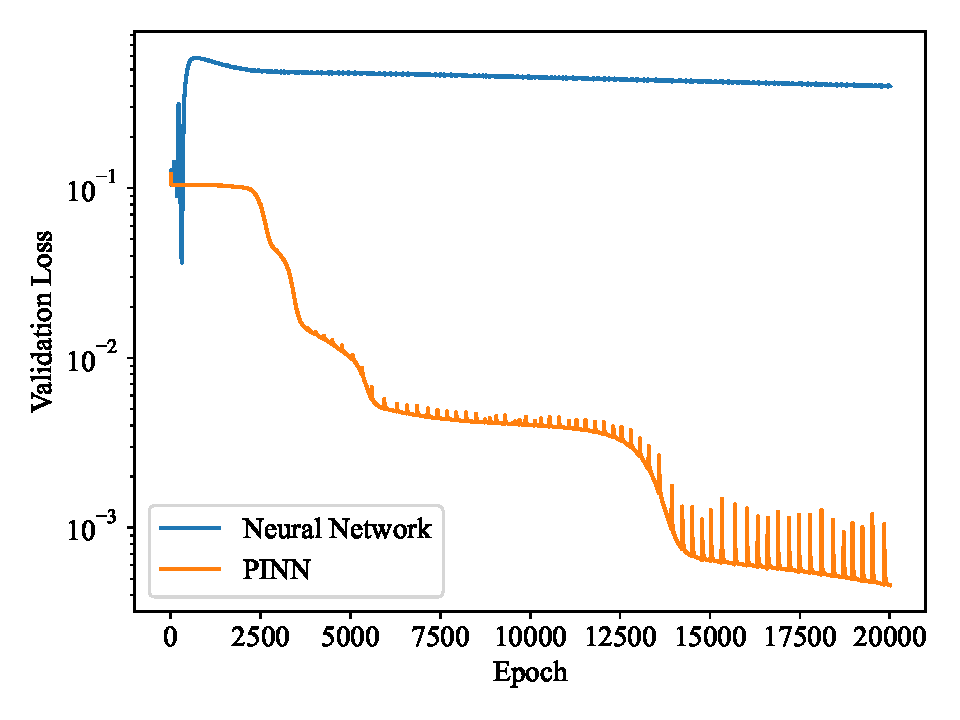
\includegraphics[width=1.0\linewidth]{Figures/InitialExperiments/msd_val_loss.pdf}
    \caption{Validation loss from a standard neural network and a PINN trained on a mass spring damper system.}
    \label{fig:msd_val_loss}
\end{figure}

Next up, two identical PINNs were trained on the same mass spring damper datapoints as before, except now that one PINN has $N_f = 100$ collocation points as before, and the other has $N_f = 30$ collocation points. Both sets of collocation points are sampled from the same time interval uniformly. The output trajectories are visualized in Figure \ref{fig:msd_pinns}.

\begin{figure}[H]
    \centering
    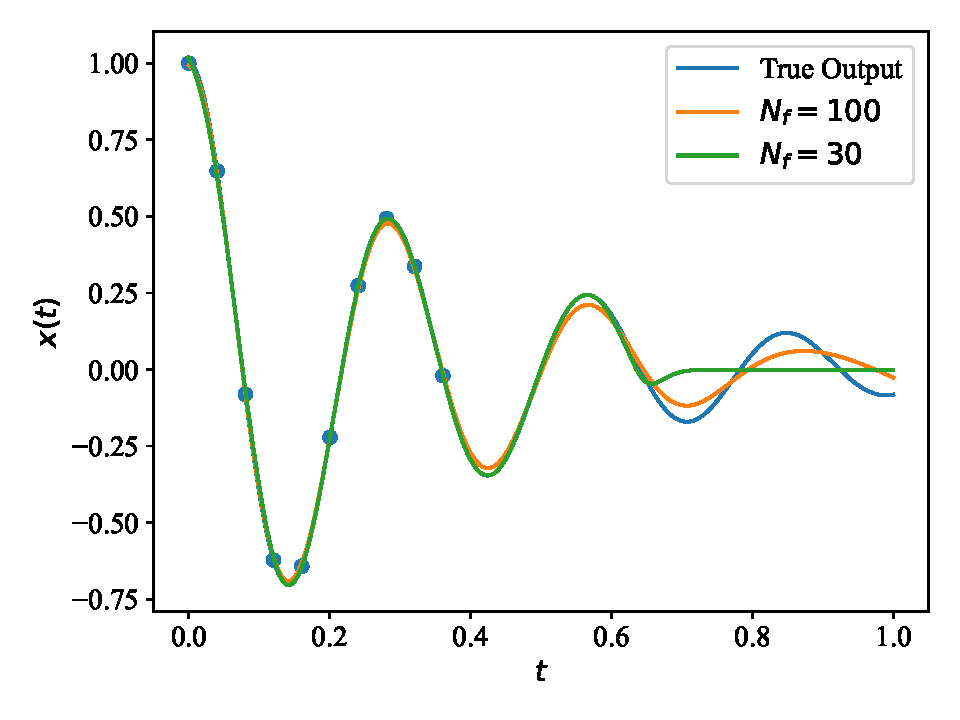
\includegraphics[width=1.0\linewidth]{Figures/InitialExperiments/msd_pinns.pdf}
    \caption{Output trajectories from two PINNs trained on a mass spring damper system with different number of collocation points. Datapoints are highlighted as blue dots.}
    \label{fig:msd_pinns}
\end{figure}

Both PINNs are following the true output for some time after the training data ends, but it can be seen that the PINN with the most collocation points is also the one that generalizes better. This could indicate that increasing the number of points leads to a more robust model in general. One drawback of increasing the points however is the computational training time as the model has to be differentiated with respect to the prior ODE at every point. The validation loss from training these two PINNs are shown in Figure \ref{fig:msd_loss_pinns}.

\begin{figure}[H]
    \centering
    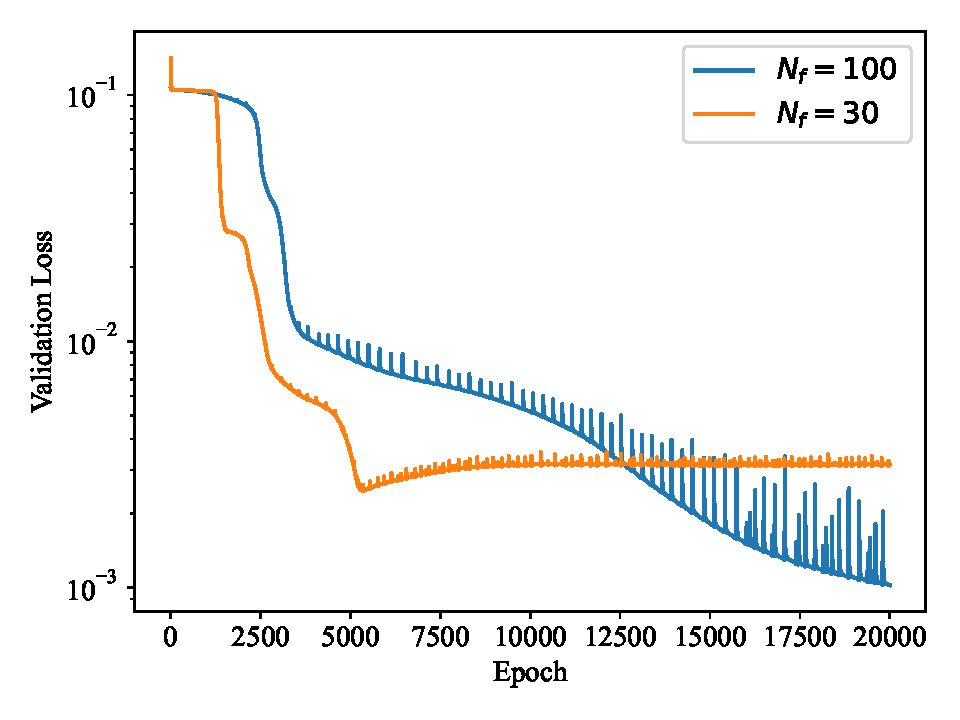
\includegraphics[width=1.0\linewidth]{Figures/InitialExperiments/msd_loss_pinns.pdf}
    \caption{Validation loss two PINNs trained on a mass spring damper system with different number of collocation points. Datapoints are highlighted as blue dots.}
    \label{fig:msd_loss_pinns}
\end{figure}

It can be seen that not only is the PINN with fewer collocation points much faster to train in terms of CPU time, but it also escaped the local minima $x(t) = 0$ faster. However, with enough training steps the PINN with more points does catch up and ends up at an even lower validation loss. The robustness of a PINN model is therefore dependent exclusively on the amount of time willing to spend on training. It also appears that if the number of training steps are expensive enough to be limited it is beneficial to reduce the number of collocation points, or put invertedly, the number of collocation points must increase alongside training epochs to maintain the relative robustness.

\subsubsection{Nonlinear ODE}

A standard neural network and a PINN trained on the Van der Pol oscillator and computing the output trajectories are shown in Figure \ref{fig:vdp}. Both models are able to hit every datapoint perfectly, as expected with enough training. In this case the dynamics are more complicated which results in the standard neural network overfitting heavily on the relatively few datapoints in comparison. This could be solved by using more data, and possibly reducing the model complexity, but it will still struggle to generalize outside the training interval as seen in the previous experiment.

The PINN is following the true output almost perfectly with the same model complexity and datapoints as the standard neural network. As the dynamics are more complicated than the mass spring damper it is easier to train a PINN and can be done in fewer epochs and without trading off the data loss.

\begin{figure}[H]
    \centering
    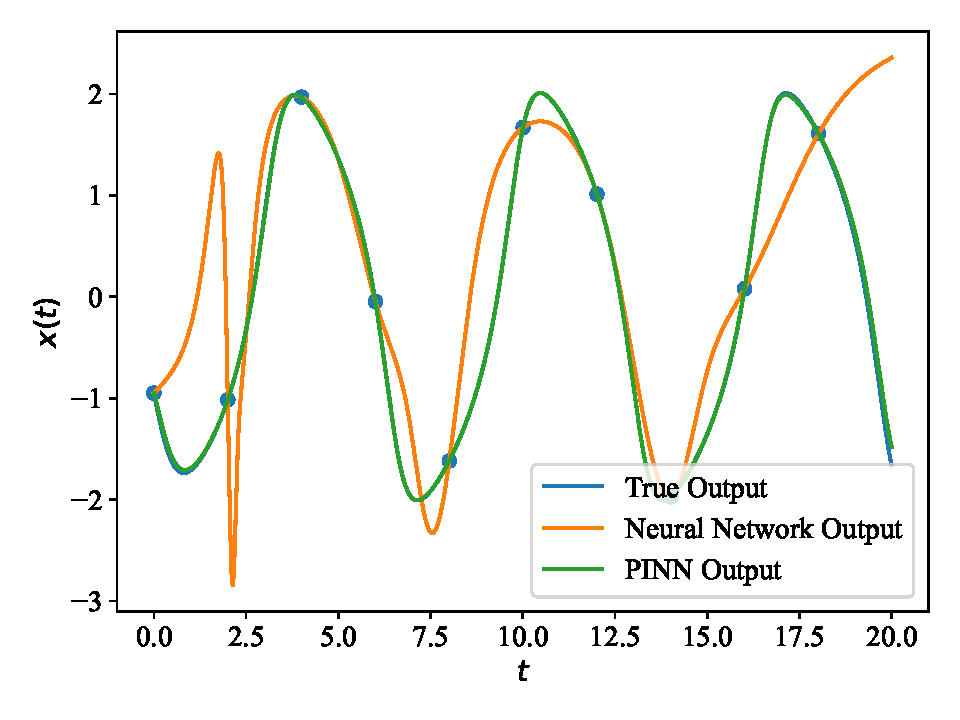
\includegraphics[width=1.0\linewidth]{Figures/InitialExperiments/vdp.pdf}
    \caption{Output trajectories from a standard neural network and a PINN trained on a Van der Pol oscillator system. Datapoints are highlighted as blue dots.}
    \label{fig:vdp}
\end{figure}

\subsubsection{Time-varying ODE}

Training a PINN on the dynamics of the Riccati equation (\ref{eq:riccati}) without using any data at all results in Figure \ref{fig:riccati_physics}. As there is a time-varying equilibrium point at $x(t) = - \sqrt{t}$ which every trajectory converges to, the PINN trajectory also converges to this. The first initial value of the PINN trajectory is a random point coming from the initialization of the parameters.

\begin{figure}[H]
    \centering
    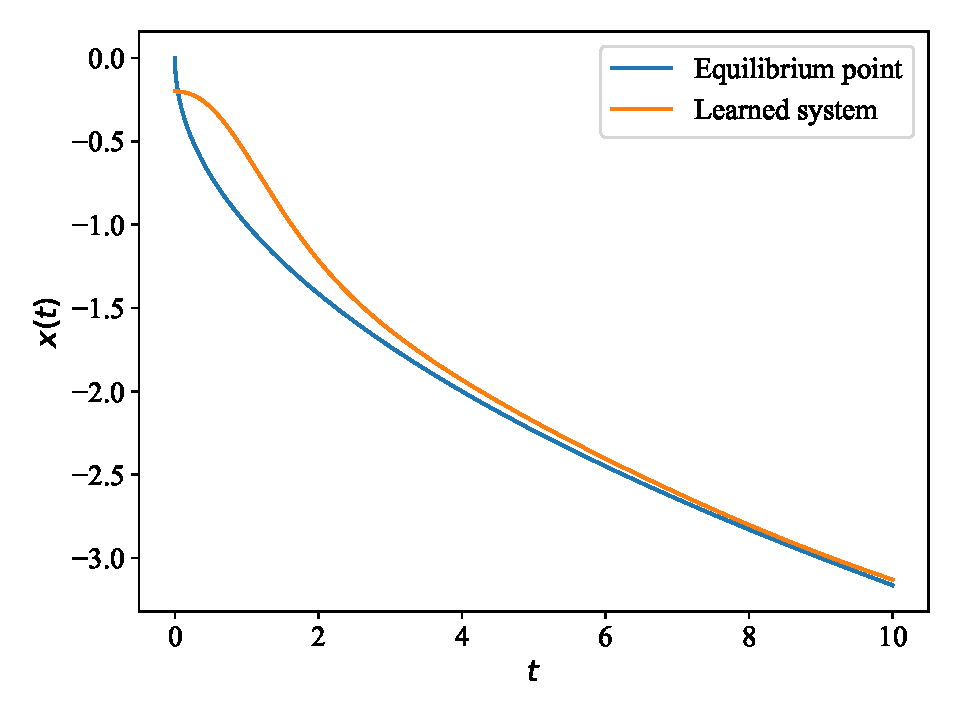
\includegraphics[width=1.0\linewidth]{Figures/InitialExperiments/riccati_physics.pdf}
    \caption{Training a physics informed neural network to learn the output trajectory of a Riccati equation without any datapoints.}
    \label{fig:riccati_physics}
\end{figure}

Adding an initial condition as a single datapoint to the PINN training results in the trajectory visualized in Figure \ref{fig:riccati}.

\begin{figure}[H]
    \centering
    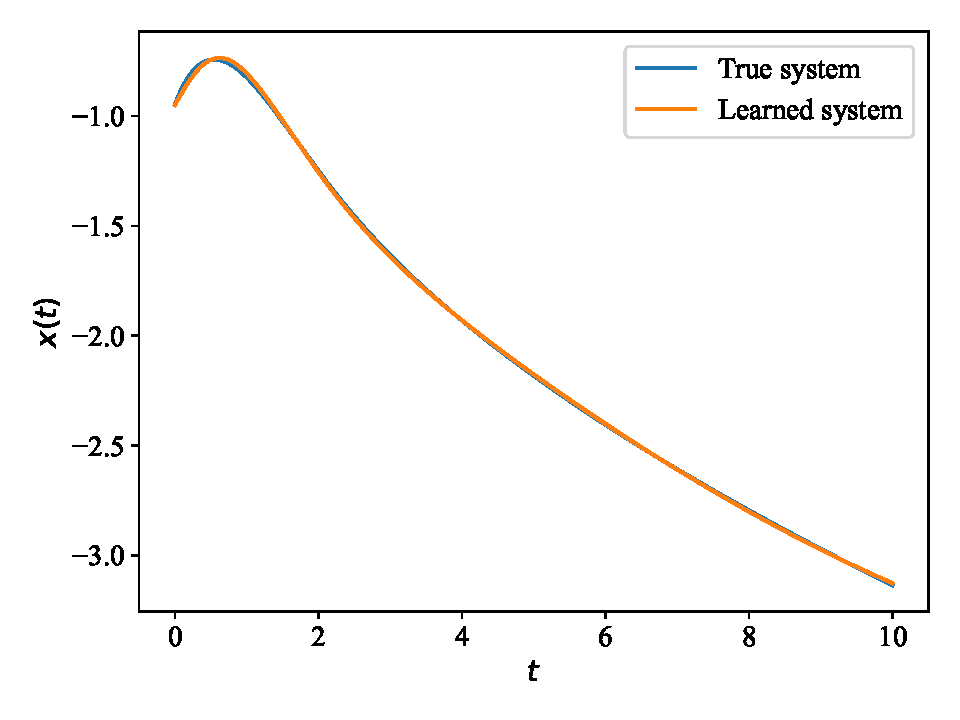
\includegraphics[width=1.0\linewidth]{Figures/InitialExperiments/riccati.pdf}
    \caption{Training a physics informed neural network to learn the output trajectory of a Riccati equation based on a single datapoint.}
    \label{fig:riccati}
\end{figure}

The PINN is now following the true system almost perfectly for as long as the collocation points were sampled from. The result was also reached in only 1000 epochs, compared to the 20000 epochs necessary for the mass spring damper. It appears that more complicated dynamics makes it possible to get away with less data while still learning a robust model. In many real life systems modeled as nonlinear ODEs, small modeling inaccuracies can cause the system to behave in wildly unexpected ways. This is a major drawback of many nonlinear control systems \cite{nonlinearsystems} and must also be accounted for when training PINNs on prior dynamics.

\subsubsection{1D Linear PDE}

The PINN output after training on the 1-dimensional heat equation is shown in Figure \ref{fig:heat1d}. The initial and boundary conditions are learned accurately, as well as the general trend of the heat dissipation. The output is almost identical to the true solution shown in Figure \ref{fig:heat1d_true}. Computing the validation loss of the PINN can be done by comparing outputs against the true analytical solution throughout the whole spatio-temporal domain with the MSE loss function. The final validation loss value after training is complete is as low as: $6.2244 \cdot 10^{-5}$, which confirms the visual comparison that the PINN has learned the true system well.

\begin{figure}[H]
    \centering
    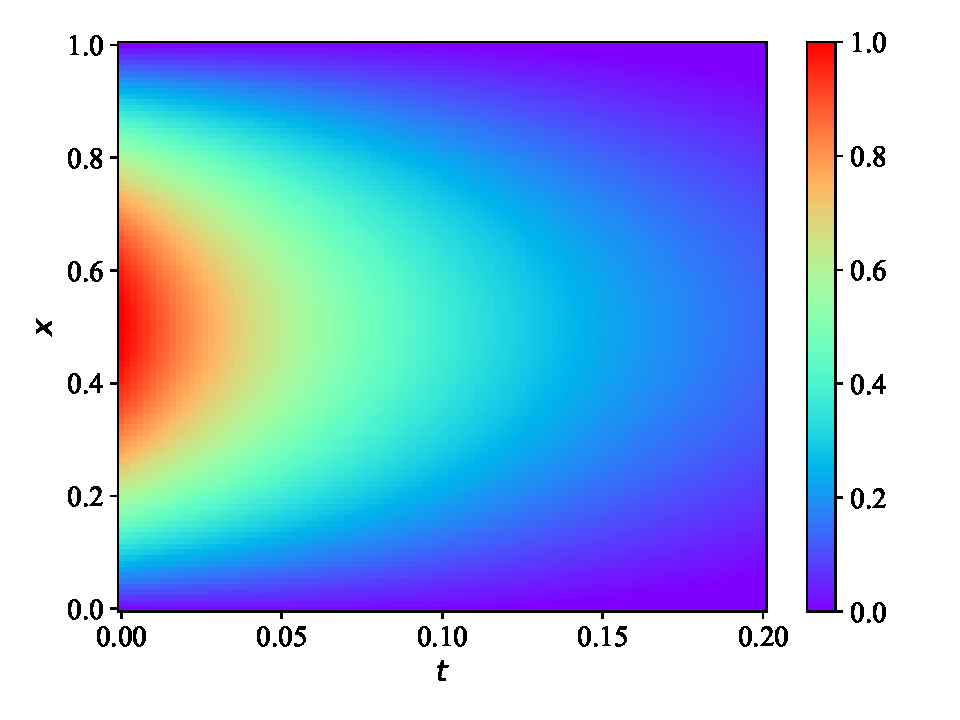
\includegraphics[width=1.0\linewidth]{Figures/InitialExperiments/heat1d.pdf}
    \caption{PINN output after training on a 1-dimensional heat equation.}
    \label{fig:heat1d}
\end{figure}

The 1-dimensional heat equation is a relatively simple PDE so it is not surprising that the PINN is learning without any difficulties. It is also much easier to learn compared to simple ODEs, using fewer training epochs. The training data also consists entirely of points sampled from the boundary and initial conditions, which can be compared to the single datapoint used when training on the time-varying ODE. Adding interior points would make the training even easier and faster to converge.

\subsubsection{2D Linear PDE}

The setup now is identical to the previous experiment on the heat equation with the addition of an extra dimension. The extra dimension also requires more collocation points to fight back against the curse of dimensionality. The trained PINN output is seen in Figure \ref{fig:heat2d} and is again able to learn the initial and boundary conditions well alongside learning the heat dissipation.

\begin{figure}[H]
     \centering
     \begin{subfigure}[b]{0.45\textwidth}
         \centering
         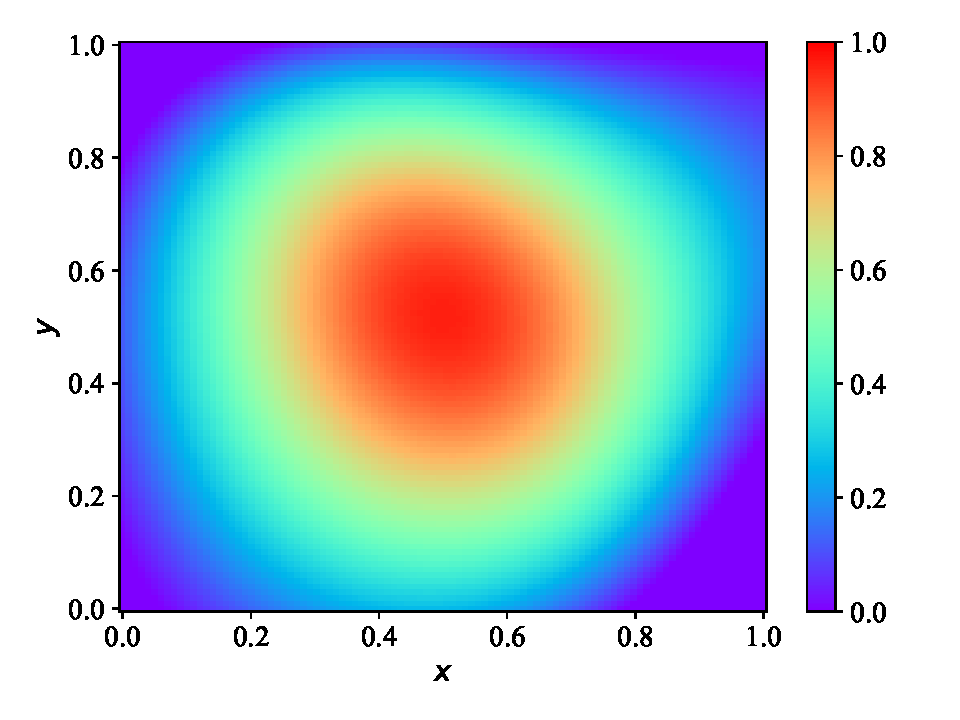
\includegraphics[width=\textwidth]{Figures/InitialExperiments/heat2d_1.pdf}
         \caption{$t = 0$}
         \label{fig:heat2d_1}
     \end{subfigure}
     \hfill
     \begin{subfigure}[b]{0.45\textwidth}
         \centering
         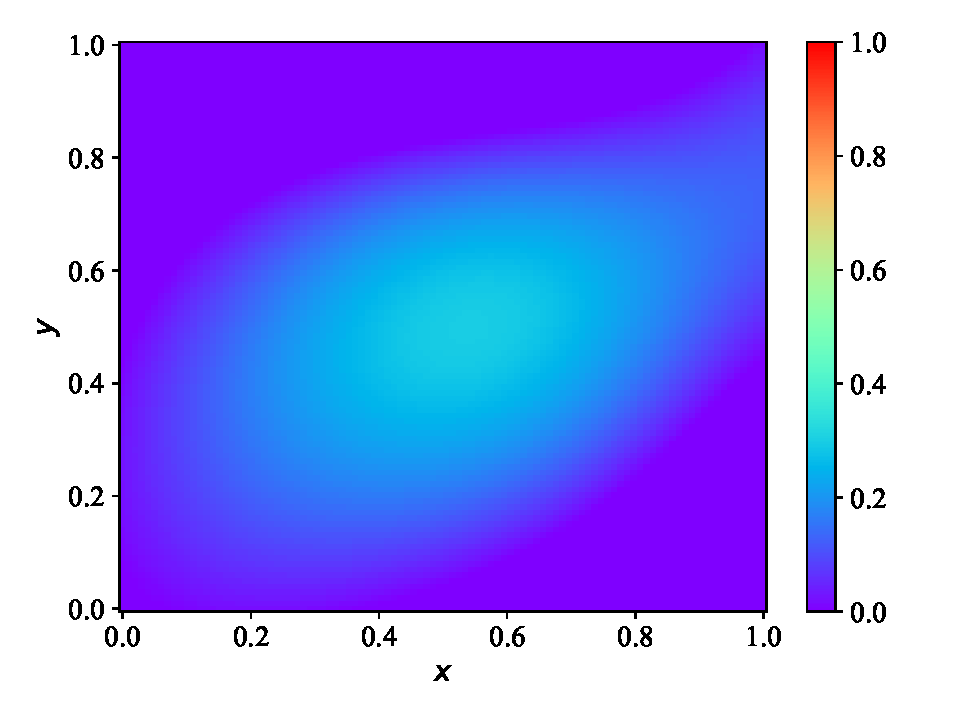
\includegraphics[width=\textwidth]{Figures/InitialExperiments/heat2d_2.pdf}
         \caption{$t = 0.067$}
         \label{fig:heat2d_2}
     \end{subfigure}
     \vskip\baselineskip
     \begin{subfigure}[b]{0.45\textwidth}
         \centering
         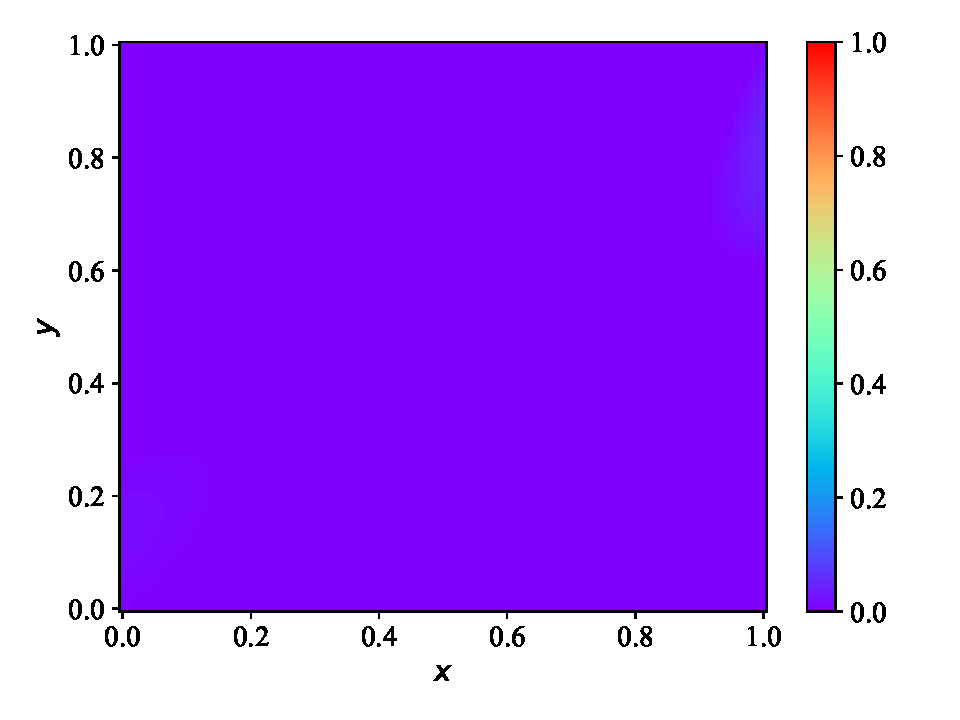
\includegraphics[width=\textwidth]{Figures/InitialExperiments/heat2d_3.pdf}
         \caption{$t = 0.133$}
         \label{fig:heat2d_3}
     \end{subfigure}
     \hfill
     \begin{subfigure}[b]{0.45\textwidth}
         \centering
         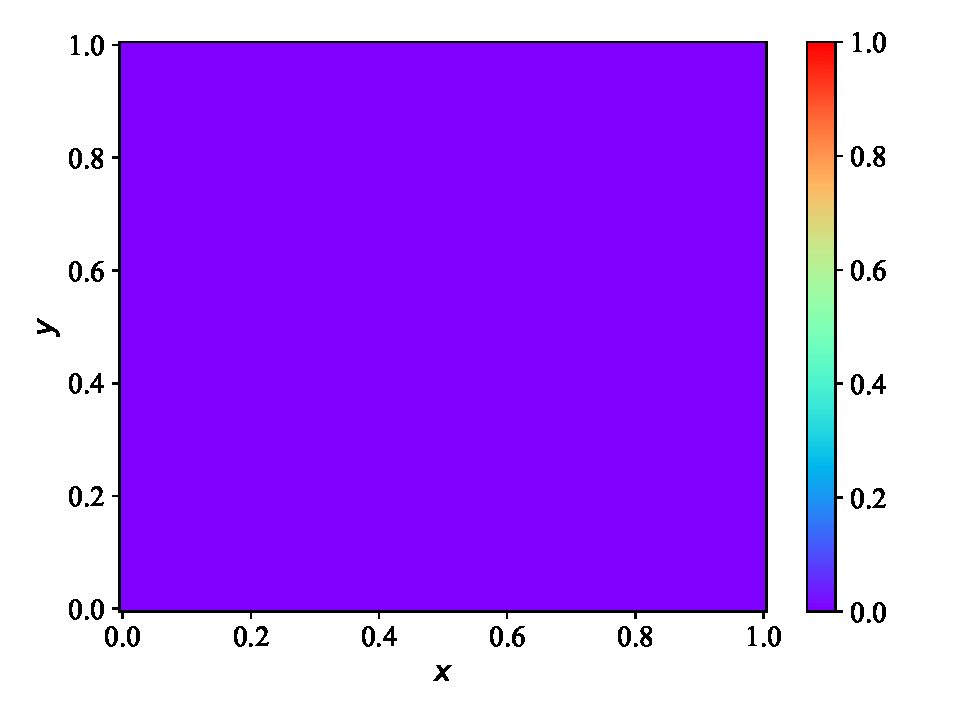
\includegraphics[width=\textwidth]{Figures/InitialExperiments/heat2d_4.pdf}
         \caption{$t = 0.2$}
         \label{fig:heat2d_4}
     \end{subfigure}
    \caption{PINN output after training on a 2-dimensional heat equation.}
    \label{fig:heat2d}
\end{figure}

Compared to the true solution it is very similar to the true solution, which is also confirmed by looking at the final validation loss at: $
0.0405$. It is however not as close to the true solution as the 1-dimensional case. The two experiments were trained on the same number of epochs, but even with the increased collocation points it is still not quite as accurate. The PINN might be trained for longer on even more collocation points to overcome this. It could also be beneficial to replace the optimizer with a better one, as was done for the data-driven discovery experiment. This does however show that even going from one to two dimensions on a simple PDE makes things much more difficult to train on.

\subsubsection{Nonlinear PDE}

At first all experiments were done using collocation points placed at a linearly spaced grid in the spatio-temporal domain, and the Adam optimizer for the training. However, the resulting output of training a PINN on the Burgers' equation was not accurate at all and seemed to be impossible with that setup. The collocation points were then changed to being sampled uniformly instead, which was also used for the previously discussed experiments, and the L-BFGS optimizer introduced here for the Burgers' equation.

Training a PINN with the improved setup worked, and the output now learns the characteristic shock formation of the Burgers' equation. This can be seen in Figure \ref{fig:burger}. As Burgers' equation is difficult to solve analytically it is also difficult to properly validate the solution without relying on numerical methods for solving PDEs. In this case, the PINN output was compared visually against the output from the paper by the original authors of the PINN framework \cite{pinn1}. Vertical slices at specific points in time of the output are also visualized separately in Figure \ref{fig:burger_slice}. This final experiment demonstrates the importance of having enough collocation points and a better optimizer for learning more difficult PDEs.

\begin{figure}[H]
    \centering
    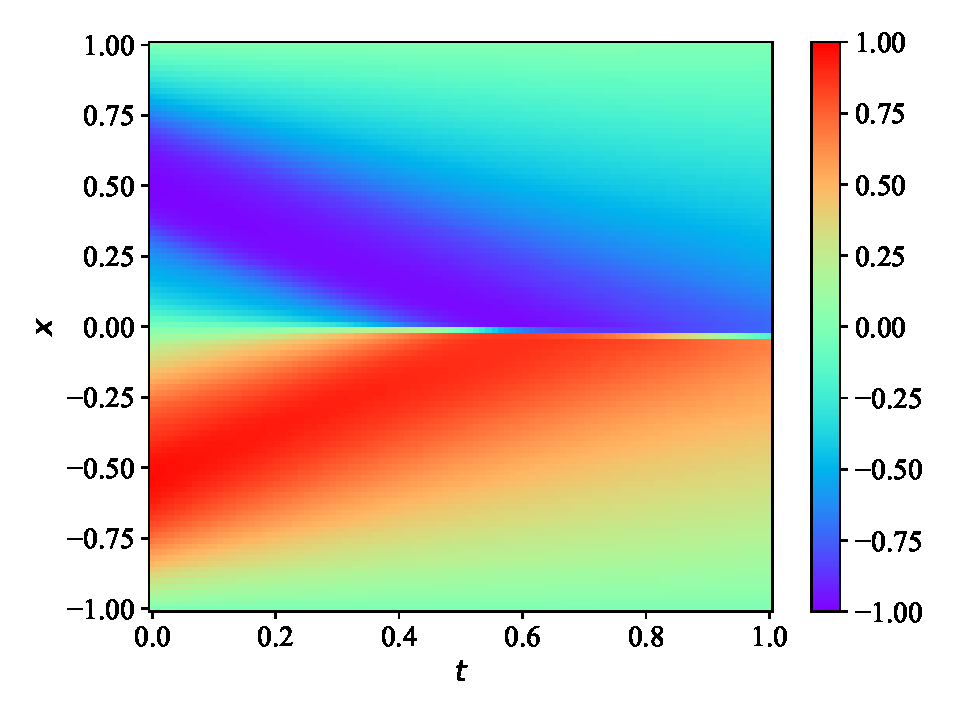
\includegraphics[width=1.0\linewidth]{Figures/InitialExperiments/burger.pdf}
    \caption{PINN output after training on a Burgers' equation.}
    \label{fig:burger}
\end{figure}

\begin{figure}[H]
     \centering
     \begin{subfigure}[b]{0.45\textwidth}
         \centering
         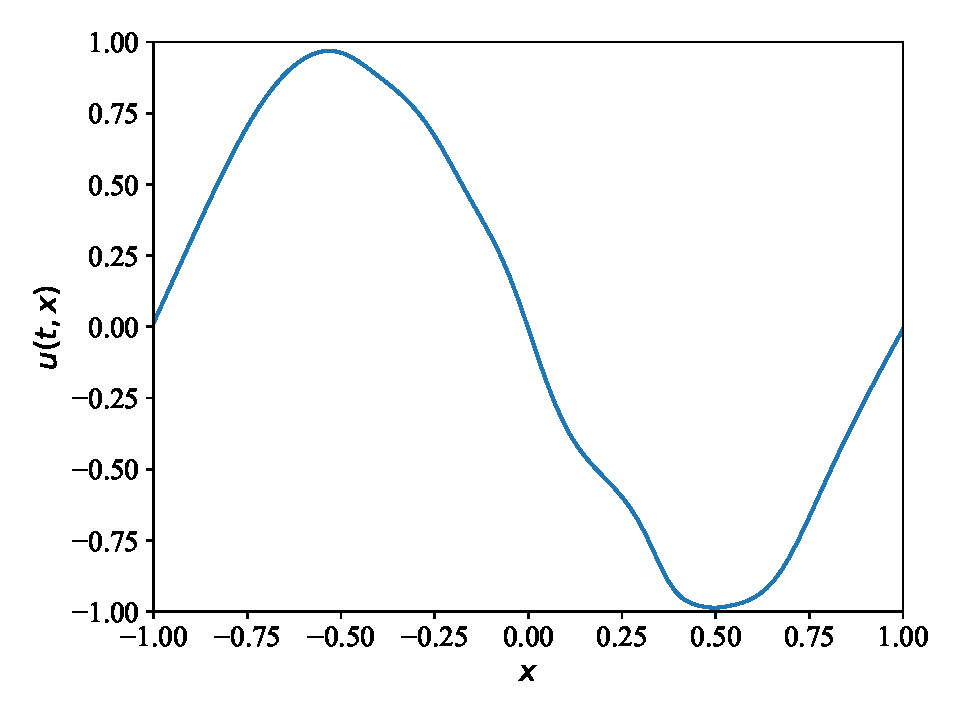
\includegraphics[width=\textwidth]{Figures/InitialExperiments/burger_slice1.pdf}
         \caption{$t = 0$}
         \label{fig:burger_slice1}
     \end{subfigure}
     \hfill
     \begin{subfigure}[b]{0.45\textwidth}
         \centering
         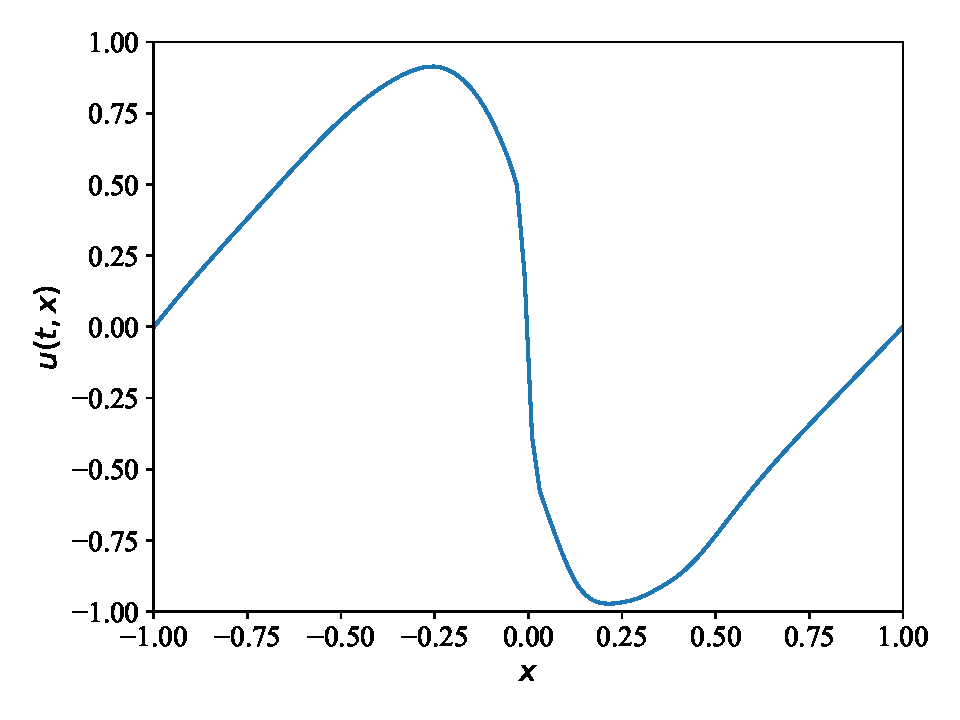
\includegraphics[width=\textwidth]{Figures/InitialExperiments/burger_slice2.pdf}
         \caption{$t = 0.333$}
         \label{fig:burger_slice2}
     \end{subfigure}
     \vskip\baselineskip
     \begin{subfigure}[b]{0.45\textwidth}
         \centering
         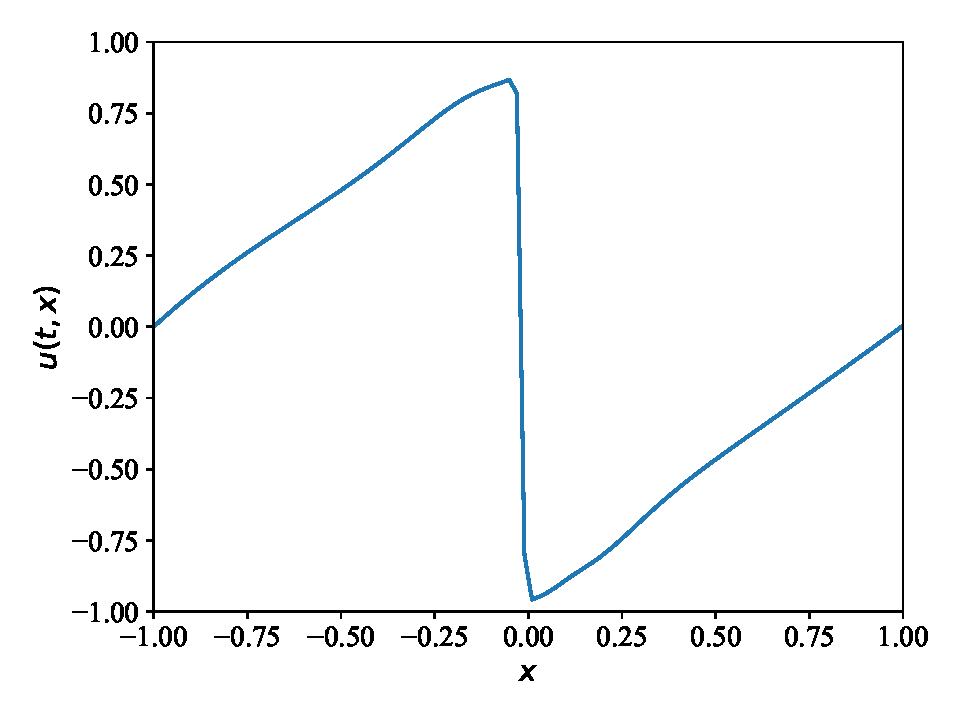
\includegraphics[width=\textwidth]{Figures/InitialExperiments/burger_slice3.pdf}
         \caption{$t = 0.667$}
         \label{fig:burger_slice3}
     \end{subfigure}
     \hfill
     \begin{subfigure}[b]{0.45\textwidth}
         \centering
         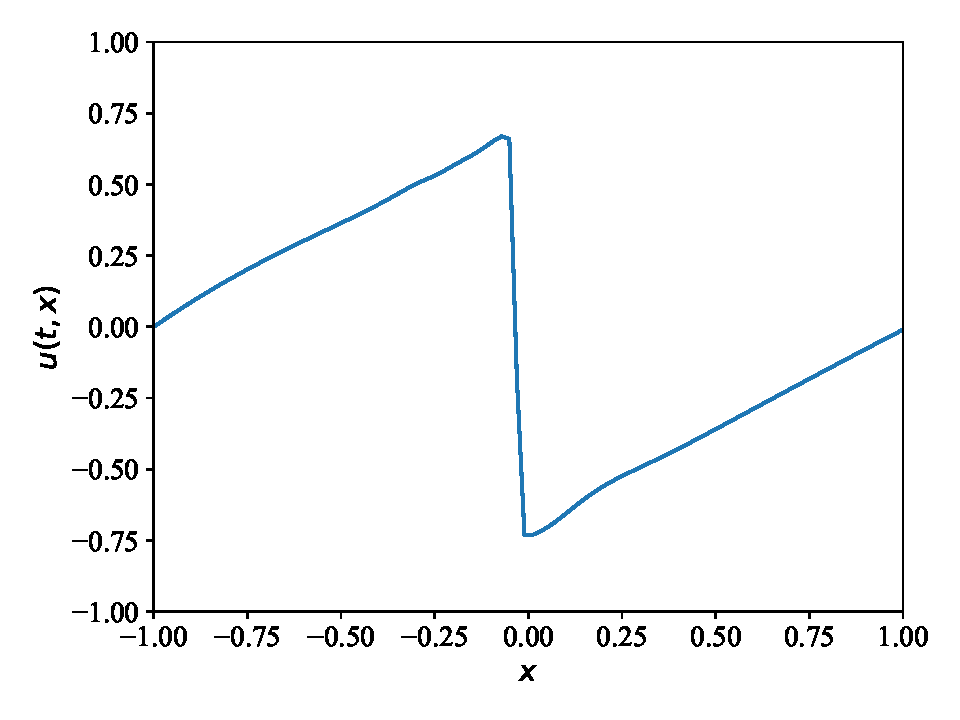
\includegraphics[width=\textwidth]{Figures/InitialExperiments/burger_slice4.pdf}
         \caption{$t = 1$}
         \label{fig:burger_slice4}
     \end{subfigure}
    \caption{Visualization of time-slices from the PINN output after training on a Burgers' equation.}
    \label{fig:burger_slice}
\end{figure}

\subsection{Data-Driven Discovery of Dynamical Systems with PINNs}

\subsubsection{1D Linear PDE}

The output from a PINN trained on the 1-dimensional heat equation is visualized in Figure \ref{fig:heat1d_discovery}. The output looks very similar to both the true solution and the previous experiment, which is also confirmed from the validation loss at: $2.0372 \cdot 10^{-5}$. The final validation loss here is even lower than the previous experiment with the known parameter, which could be a result of replacing the optimizer and increasing the amount of data to cover the interior of the domain.

\begin{figure}[H]
    \centering
    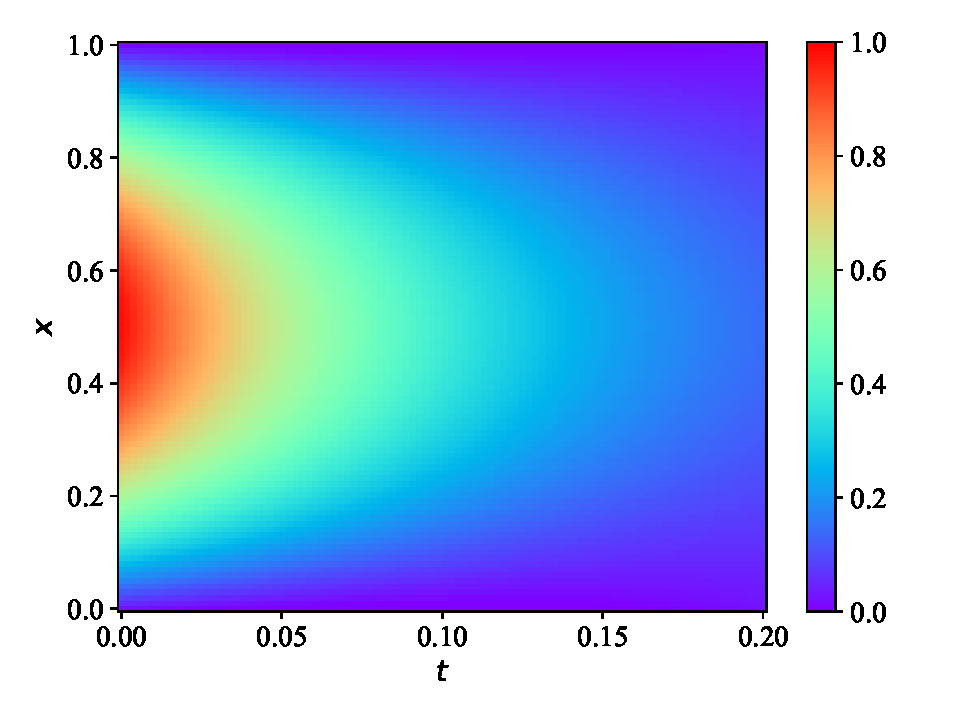
\includegraphics[width=1.0\linewidth]{Figures/InitialExperiments/heat1d_discovery.pdf}
    \caption{PINN output after training on a 1-dimensional heat equation with an unknown parameter.}
    \label{fig:heat1d_discovery}
\end{figure}

The true value of the parameter was set to $k = 1$ for simplicity, and the final estimate of the parameter after training was: $\hat{k} = 0.989268$, which is very close to the true value. An interesting thing that occasionally happened was that the estimate would converge towards $-1$ instead, which is equivalent for the heat equation (\ref{eq:heat1d}) where the parameter is squared. The initial value of the estimate was sampled from a standard normal, so it would often converge depending on which side of zero it started at. Having prior information about the parameter could be useful in this case to ensure that it converges to the correct value.

The purpose of this experiment was less about learning the output of the system with a PINN and more about discovering the structure of the underlying dynamics. Because of the increase in data quantity required it might be feasible to train a neural network on the output data without using any prior physics information, but using PINNs it is possible to both learn a representation of the output while also simultaneously estimating the unknown parameters.

\subsubsection{2D Linear PDE}

The same experiment was now repeated for the 2-dimensional heat equation, and the final output of the trained PINN is shown in Figure \ref{fig:heat2d}. The output is again very similar to the true solution and output from the previous experiment with the 2-dimensional heat equation. The final validation loss after training is: $5.2727 \cdot 10^{-5}$, which is much lower than the previous experiment with the known parameter, which again could be explained by the change of optimization algorithm and increased data quantity.

The final estimate of the parameter after training ends up at: $\hat{k} = 0.993225$ compared to the true value of $k = 1$ which means that the PINN learned the true system well. However, increasing the dimension requires significantly more data than compared to the previous 1-dimensional case, where the number of training points and collocation points is increased from 1000 to 20000. This also increases the computational cost, but the most significant drawback is the reliance on training data, as more collocation points can always be generated. Collecting data from real systems can often be difficult, so it might not always be feasible to estimate unknown parameters with this method. Although, if there exists some prior information about the value of the parameter in addition to the system dynamics this could also be incorporated into the PINN training. For example if the parameter value itself is unknown, but has a known minimum and maximum value, this prior information can be used during training by clipping the parameter value to this range after every iteration. For the heat equation specifically it can for example be assumed that the heat conductivity is a positive value, thus limiting the range from below by zero.

\begin{figure}[H]
     \centering
     \begin{subfigure}[b]{0.45\textwidth}
         \centering
         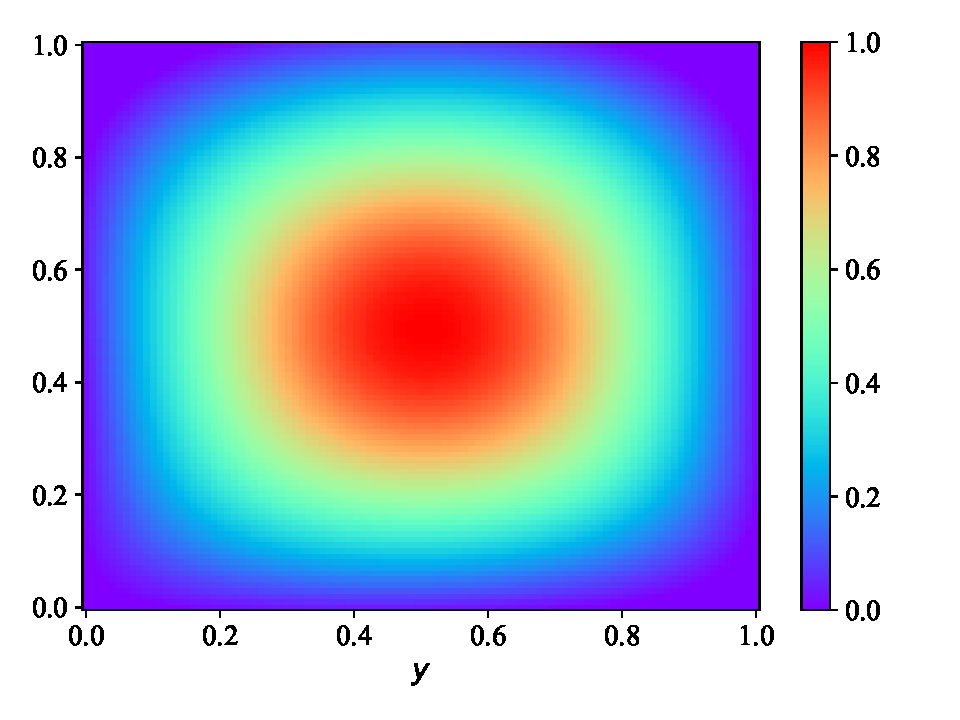
\includegraphics[width=\textwidth]{Figures/InitialExperiments/heat2d_1_discovery.pdf}
         \caption{$t = 0$}
         \label{fig:heat2d_1_discovery}
     \end{subfigure}
     \hfill
     \begin{subfigure}[b]{0.45\textwidth}
         \centering
         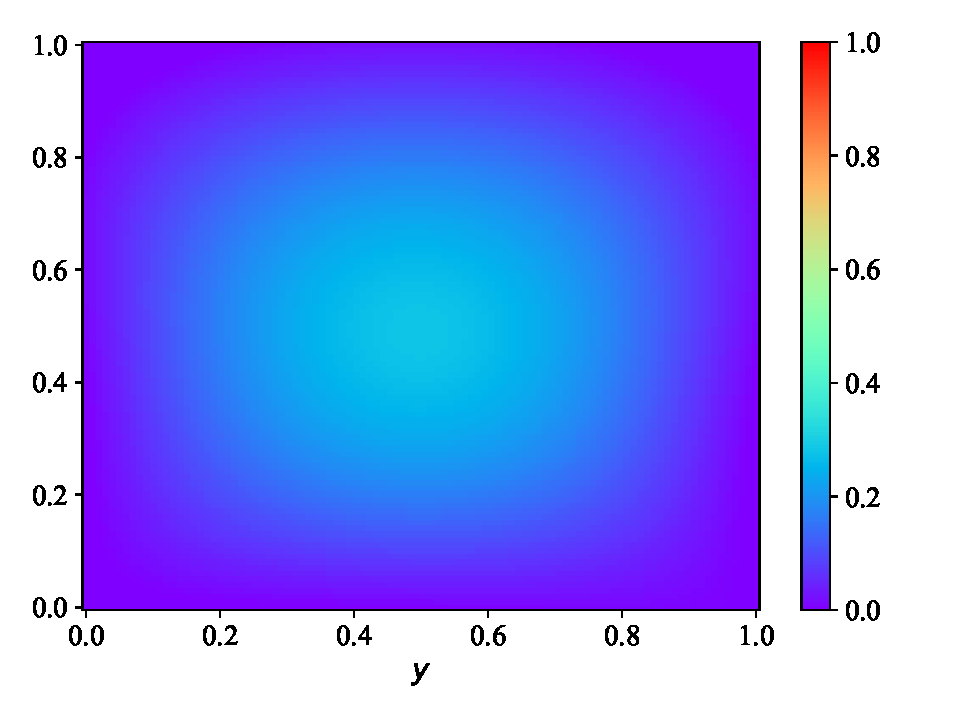
\includegraphics[width=\textwidth]{Figures/InitialExperiments/heat2d_2_discovery.pdf}
         \caption{$t = 0.067$}
         \label{fig:heat2d_2_discovery}
     \end{subfigure}
     \vskip\baselineskip
     \begin{subfigure}[b]{0.45\textwidth}
         \centering
         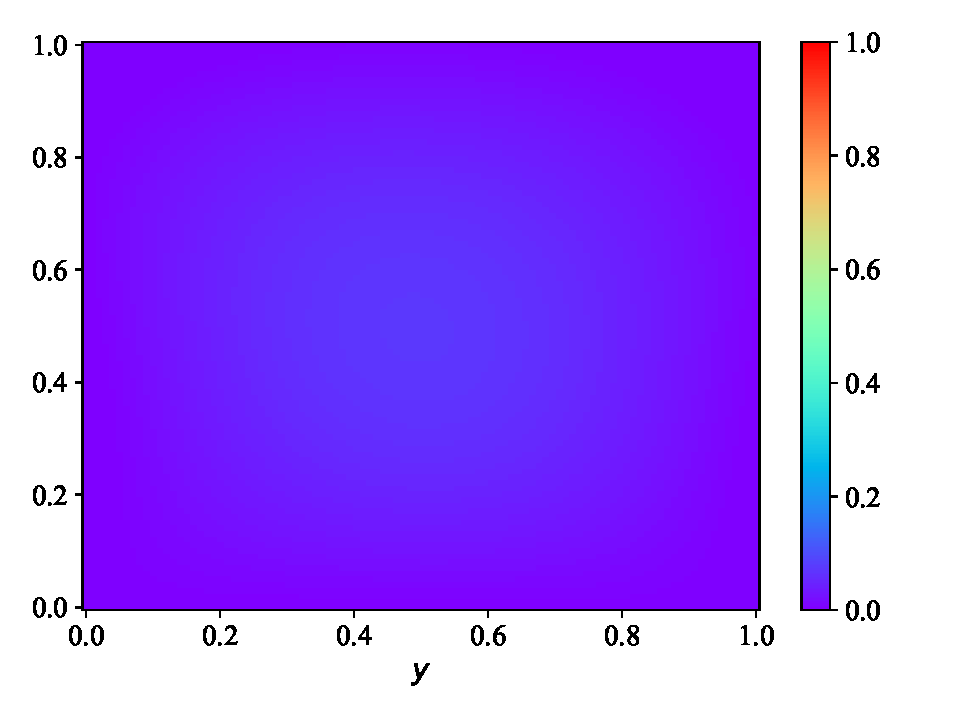
\includegraphics[width=\textwidth]{Figures/InitialExperiments/heat2d_3_discovery.pdf}
         \caption{$t = 0.133$}
         \label{fig:heat2d_3_discovery}
     \end{subfigure}
     \hfill
     \begin{subfigure}[b]{0.45\textwidth}
         \centering
         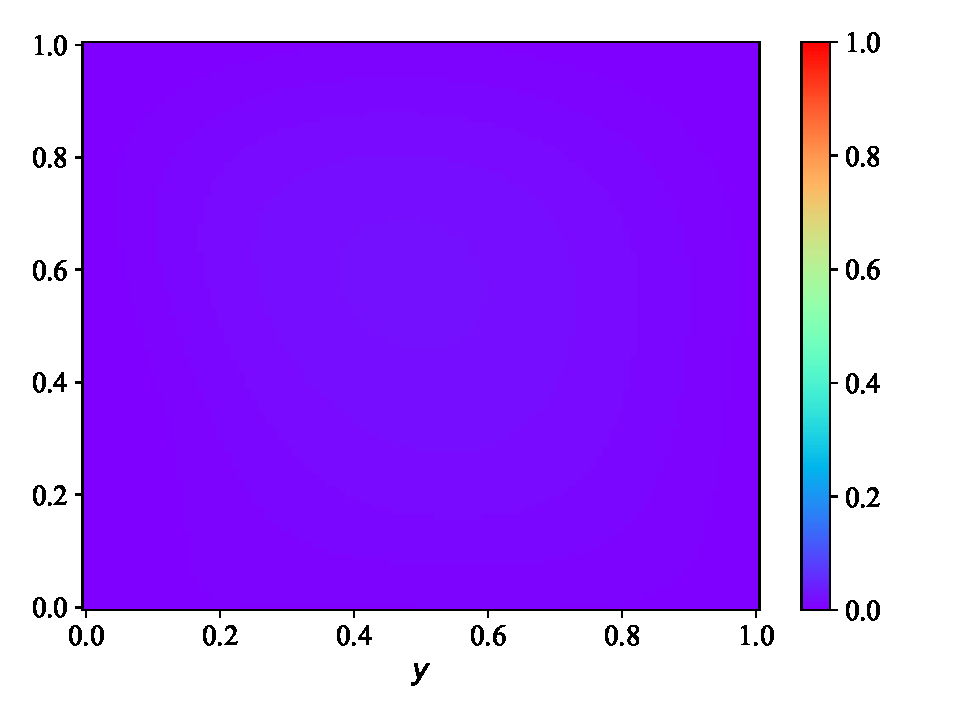
\includegraphics[width=\textwidth]{Figures/InitialExperiments/heat2d_4_discovery.pdf}
         \caption{$t = 0.2$}
         \label{fig:heat2d_4_discovery}
     \end{subfigure}
    \caption{PINN output after training on a 2-dimensional heat equation with an unknown parameter.}
    \label{fig:heat2d_discovery}
\end{figure}

\subsection{Causal Training}

\subsubsection{Simple PDE}

With all the training enhancements of the modified network structure, Fourier embeddings, causal loss with epsilon annealing and time-marching, the resulting output from solving the Burger's equation is shown in Figure \ref{fig:causal_burger}. The complete output was created by stitching together the individual outputs from the smaller submodels. The quality is seen to be much higher compared to the previous more default approach shown in Figure \ref{fig:burger}.

\begin{figure}[H]
    \centering
    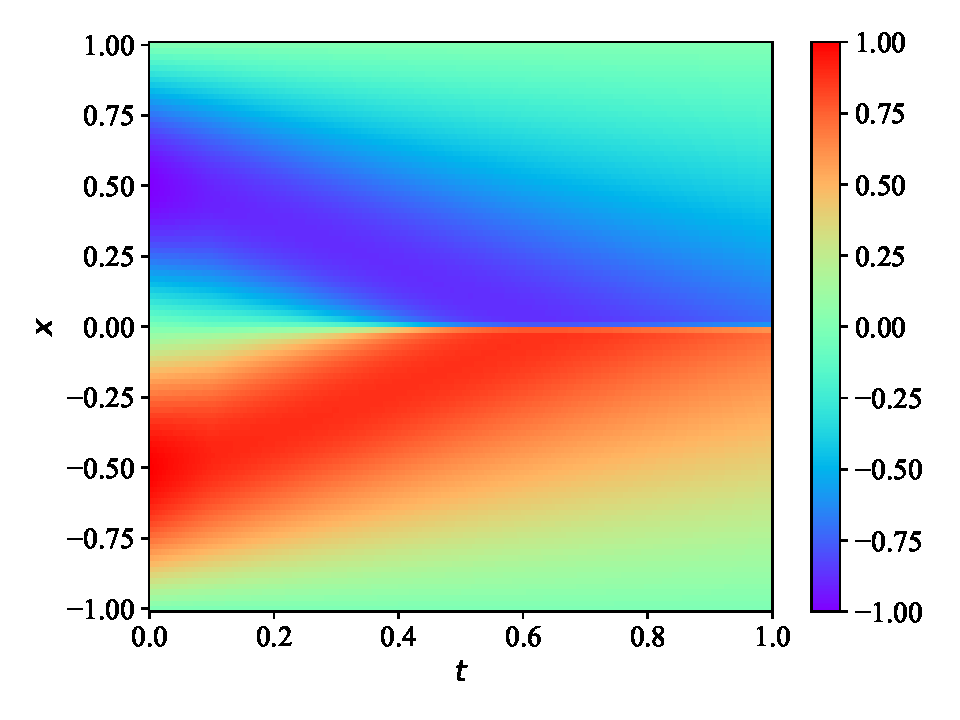
\includegraphics[width=1.0\linewidth]{Figures/IntermediateExperiments/Causality/Burger/burger.pdf}
    \caption{Burgers' equation solved with causal PINN training.}
    \label{fig:causal_burger}
\end{figure}

Visualizations of the output at specific slices in time are shown below in Figure \ref{fig:burger_slice_causal}. Comparing this to the slices from the default approach in Figure \ref{fig:burger_slice}, the plots look more smooth and symmetric, which indicates a higher accuracy.

\begin{figure}[H]
     \centering
     \begin{subfigure}[b]{0.45\textwidth}
         \centering
         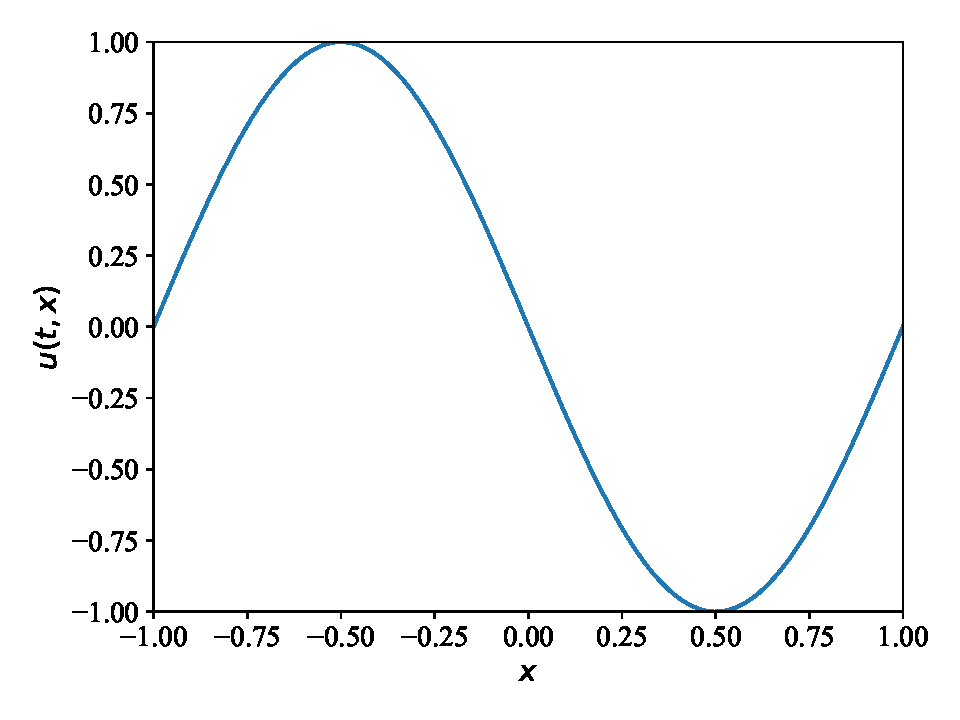
\includegraphics[width=\textwidth]{Figures/IntermediateExperiments/Causality/Burger/burger_slice1.pdf}
         \caption{$t = 0$}
         \label{fig:burger_slice1_causal}
     \end{subfigure}
     \hfill
     \begin{subfigure}[b]{0.45\textwidth}
         \centering
         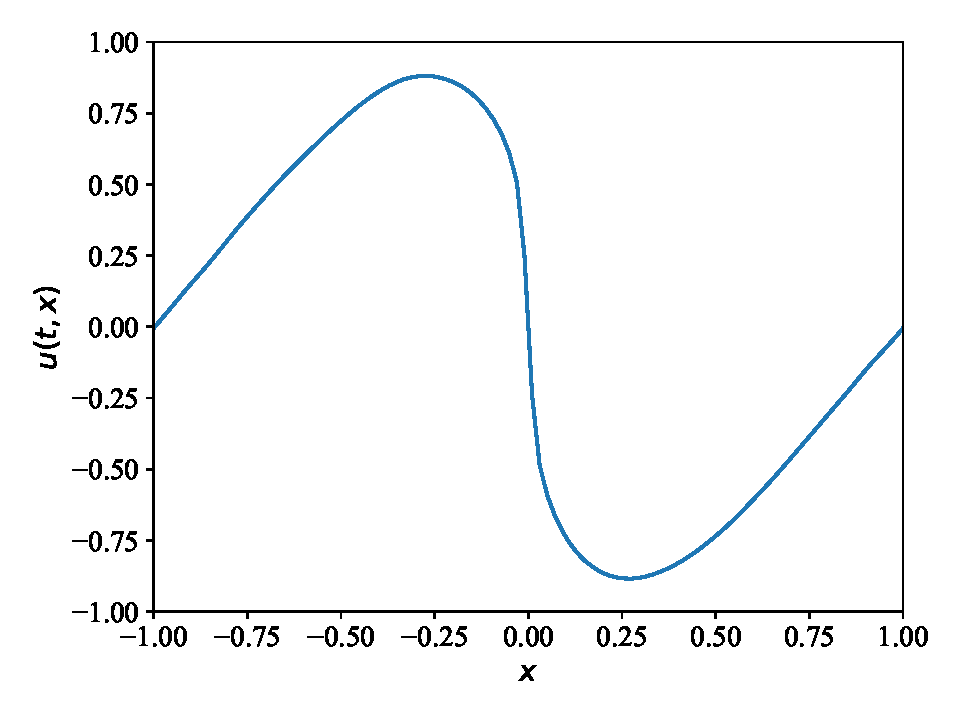
\includegraphics[width=\textwidth]{Figures/IntermediateExperiments/Causality/Burger/burger_slice2.pdf}
         \caption{$t = 0.333$}
         \label{fig:burger_slice2_causal}
     \end{subfigure}
     \vskip\baselineskip
     \begin{subfigure}[b]{0.45\textwidth}
         \centering
         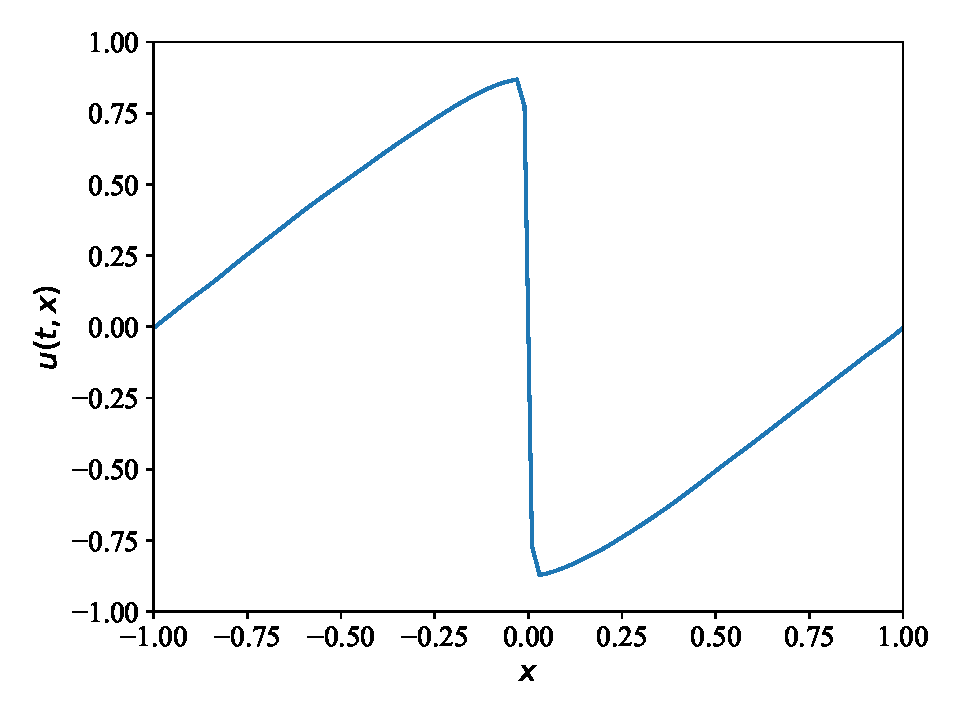
\includegraphics[width=\textwidth]{Figures/IntermediateExperiments/Causality/Burger/burger_slice3.pdf}
         \caption{$t = 0.667$}
         \label{fig:burger_slice3_causal}
     \end{subfigure}
     \hfill
     \begin{subfigure}[b]{0.45\textwidth}
         \centering
         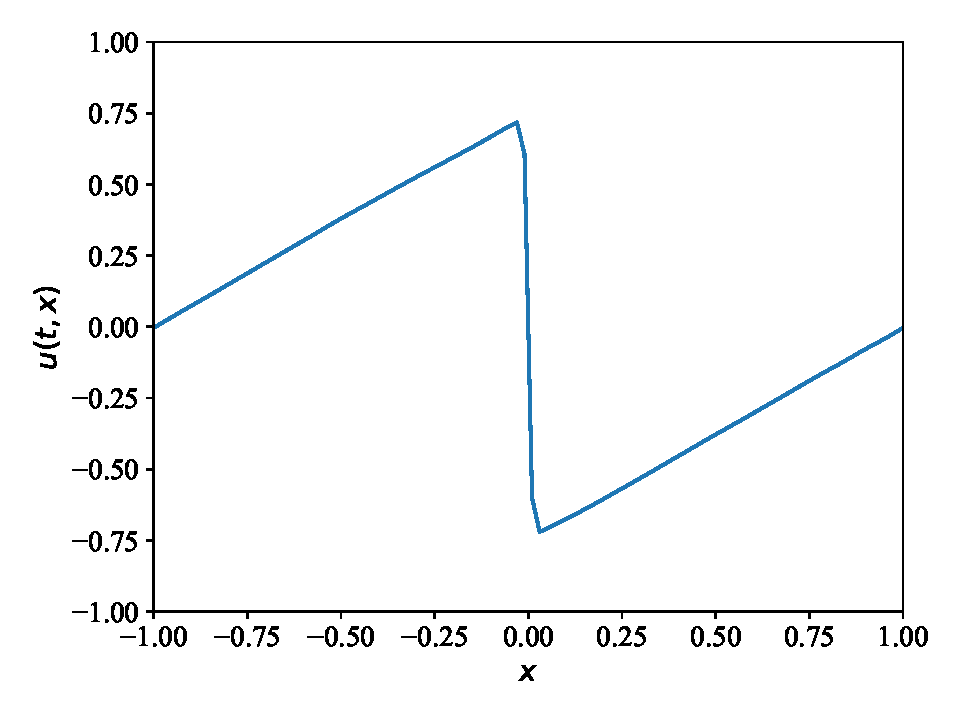
\includegraphics[width=\textwidth]{Figures/IntermediateExperiments/Causality/Burger/burger_slice4.pdf}
         \caption{$t = 1$}
         \label{fig:burger_slice4_causal}
     \end{subfigure}
    \caption{Visualization of time-slices from the PINN output after causal training on a Burgers' equation.}
    \label{fig:burger_slice_causal}
\end{figure}

The purpose of this experiment was to show that the enhancements to the PINN training process work and give accurate results. But the increased computational cost may not be worth it for all problems.

\subsubsection{Chaotic PDE}

Moving on to the more complicated Allen-Cahn equation, training a PINN without any of the enhancements will generally work very poorly. The result of doing this is not shown here, as the plot would be just tending towards zero as the time increases. However, by incorporating some of the enhancements described in the method section and training a PINN, results in the output plot shown below in Figure \ref{fig:causal_ac}.

\begin{figure}[H]
    \centering
    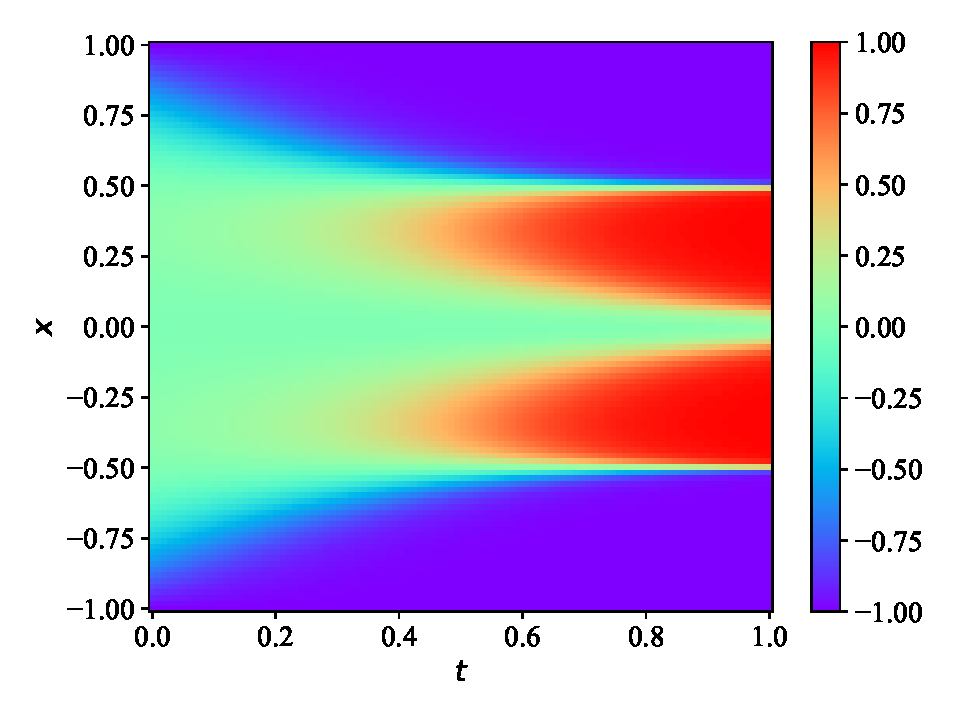
\includegraphics[width=1.0\linewidth]{Figures/IntermediateExperiments/Causality/AC/ac.pdf}
    \caption{The Allen-Cahn equation solved with causal PINN training.}
    \label{fig:causal_ac}
\end{figure}

Comparing the pointwise MSE to a numerical solver, the resulting difference becomes: $3.2457 \cdot 10^{-6}$. This is an indication that the causal training method also gives a high accuracy for chaotic systems.

Numerically solving chaotic ODEs and PDEs are often hard to do with any accuracy for longer time intervals. For a system to be chaotic it means that small differences in initial conditions results in wildly different trajectories in time. Because no numerical method is perfectly accurate, for example due to floating point arithmetic on computers, small errors will accumulate during the numerical integration. These small errors might not mean much for a non-chaotic system except that the solutions become less accurate, but for chaotic systems, the solutions will get increasingly wrong with time, making them very unreliable.

Introducing causality is a way to combat this by ensuring that sections in time are accurate enough before proceeding to the next section in time. This prevents errors from accumulating, and reduces the chaotic influence during training.

\subsection{Symbolic Operator Discovery}

\subsubsection{Nonlinear PDE}

Firstly, a PINN is trained on yet another Burgers' equation. All the same improvements as used with the causal experiment are applied here, except time-marching. Comparing the MSE loss to the numerical solver results in the difference: $2.8914 \cdot 10^{-5}$. This PINN model is then used as the ground truth to validate the accuracy of the symbolic operator discovery. This is done partially because the trained PINN model is a continuous function that can be evaluated at any point, and is therefore not restricted to the specific grid discretization as the downloaded dataset used. Additionally, having access to the model itself makes it possible to compute partial derivatives with automatic differentiation, thus making the operator accuracy more reliable. The alternative would be to use finite differences on the numerical dataset, which makes it much less reliable. This insight can also be considered a useful application of PINNs compared to numerical solvers.

Afterwards, the symbolic operator discovery is done with two different models. The first is a default PINN. The second is a PINN with the additions of the modified network structure, which seems to generally be an improvement without any noticeable drawbacks, and with a Fourier embedding to handle the known periodic boundary. The second neural network that learns the missing term of the PDE symbolically is kept as a standard neural network for both models.

Plotting the outputs of any of these models would result in yet another plot of the Burgers' equation, which has been shown many times throughout this thesis, so it was not necessary to display here yet again.

To validate the accuracy, a grid of equally spaced points are constructed over the domain to evaluate at. The networks learning the output state of the PDE are compared with the MSE against the ground truth PINN described previously. The default PINN achieves an MSE of $1.28 \cdot 10^{-4}$, and the improved PINN achieves an MSE of $7.7 \cdot 10^{-5}$, which is a slight improvement.

To validate the learned symbolic operators, automatic differentiation is used on the ground truth PINN to calculate the relevant partial derivatives. These are then evaluated on the grid of validation points. This makes it possible to explicitly calculate the ground truth operator by combining the relevant terms together. The network that learns the symbolic representation receives these true partial derivatives and state as input, and the output becomes the learned operator. The operator can then be validated by comparing with the MSE over the grid points. The first model with the standard PINN achieves an MSE of $0.286$, and the model with the improved PINN achieves an MSE of $0.194$. The improved PINN still has a slight improvement, but neither of the models appear particularly accurate in this case.

So even though both models get a relatively accurate representation of the output, they appear to not learn the symbolic expression for the unknown term very well. Although the MSE values are not necessarily that big either, and it is to a certain extent dependent on the true scale of the values of the system. This can also happen because the MSE is computed as the mean over the validation points. And for Burgers' equation in particular, as there develops a discontinuity along the origin, the derivative at that point approaches infinity as time increases. This value might get large enough to run into numerical errors, but this was not investigated thoroughly. A potential solution could be to take the median value of the MSE instead of the mean, as it is more outlier resistant. But the conclusion is anyway that it is difficult to verify the accuracy of the learned unknown term.

As the two networks are trained together, the outputs from the symbolic network are used to calculate the physics informed loss also during training. If the network was set to a constant zero, then the physics informed loss would not reflect the true PDE as there is a term missing from the equation. Therefore it means that even though the learned symbolic operator in this case might not be that accurate, it is still accurate enough to allow the other network to represent the output state of the system. It is also possible that simply tuning the hyperparameters further would result in a more accurate expression for the unknown term.

\subsection{Solving PDE-Constrained Optimal Control Problems}

\subsubsection{Flux Control}

The output state of the trained PINN can be seen below in Figure \ref{fig:laplace_optimal_control}. The boundary condition when $y = 0$ seems to be satisfied relatively well along with periodic boundary in the x-direction.

\begin{figure}[H]
    \centering
    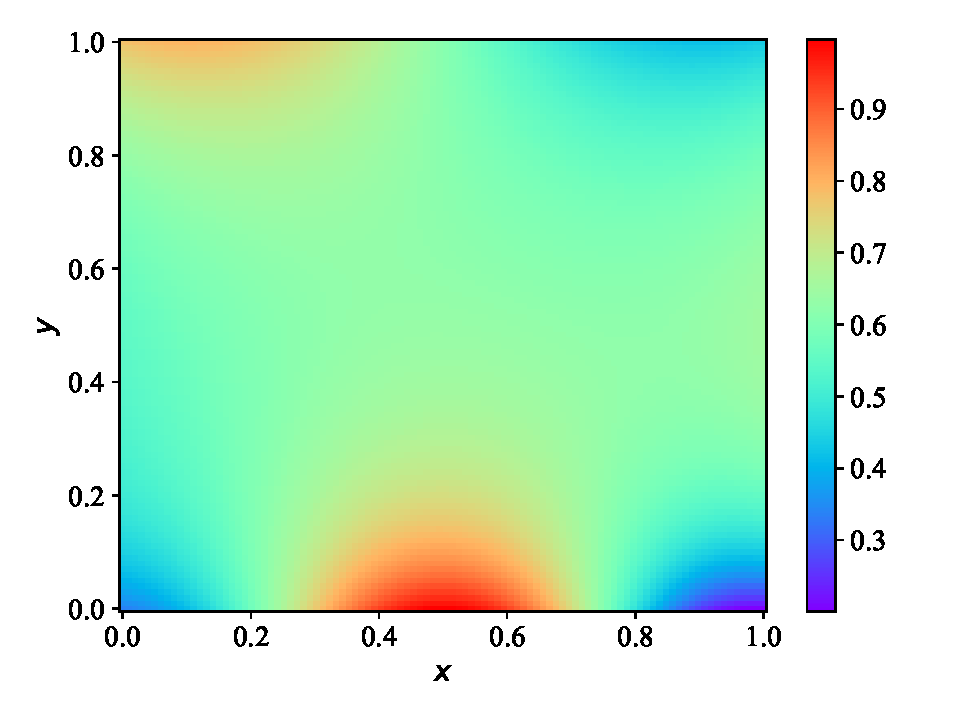
\includegraphics[width=1.0\linewidth]{Figures/IntermediateExperiments/OptimalControl/laplace_optimal_control.pdf}
    \caption{PINN output of the solution to the optimal control problem on Laplace's equation.}
    \label{fig:laplace_optimal_control}
\end{figure}

The learned control input is displayed in Figure \ref{fig:laplace_optimal_control_control}, and is working as the boundary on the top side of the domain when $y = 1$. Verifying that the flux in the y direction goes to the desired flux is not obvious from looking at any of these plots, and must be verified in another way.

\begin{figure}[H]
    \centering
    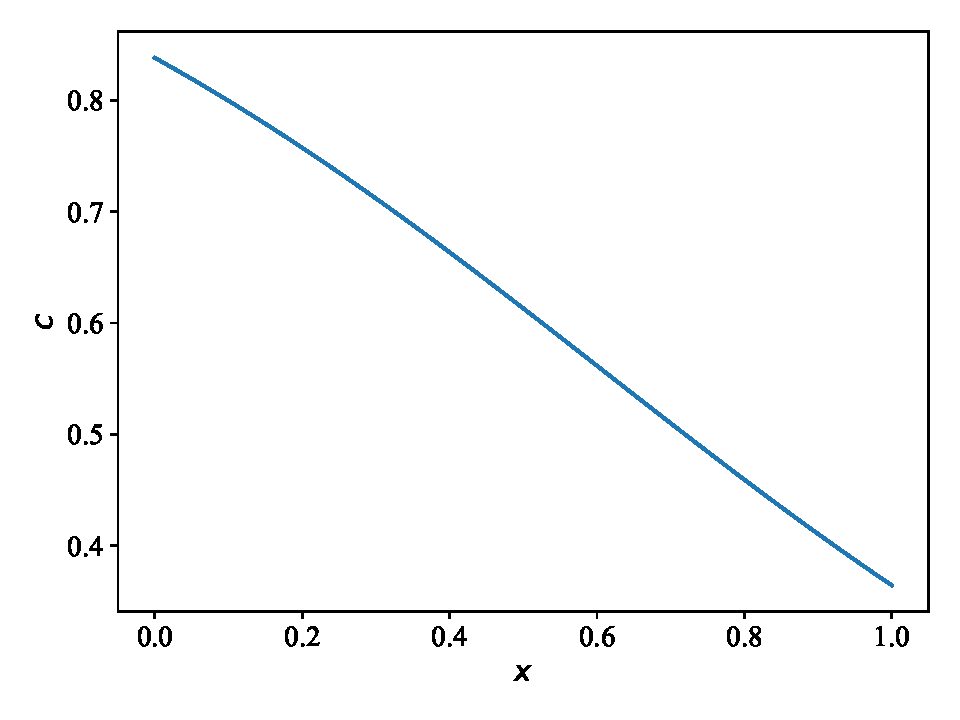
\includegraphics[width=1.0\linewidth]{Figures/IntermediateExperiments/OptimalControl/laplace_optimal_control_control.pdf}
    \caption{Learned control policy to the optimal control problem on Laplace's equation.}
    \label{fig:laplace_optimal_control_control}
\end{figure}

As both networks are trained together, they will have to learn to satisfy boundary and physics loss in addition to minimizing the objective function. By looking at the training loss values, they should all go to zero to perfectly represent the true solution to the optimal control problem. The individual training losses are shown in Figure \ref{fig:laplace_optimal_control_losses}.

It can be seen that the cost value corresponding to the objective function is prioritized during training, which makes sense due to its higher relative weighting. It also shows that the boundary loss and physics loss are much higher relatively. This can partially be explained because the periodic boundary condition is not possible to satisfy with the learned control policy in Figure \ref{fig:laplace_optimal_control_control}, as that is also not periodic. Can also see that the losses converge after around 4000 epochs to a local minima, which is because the L-BFGS method doesn't use any momentum.

\begin{figure}[H]
    \centering
    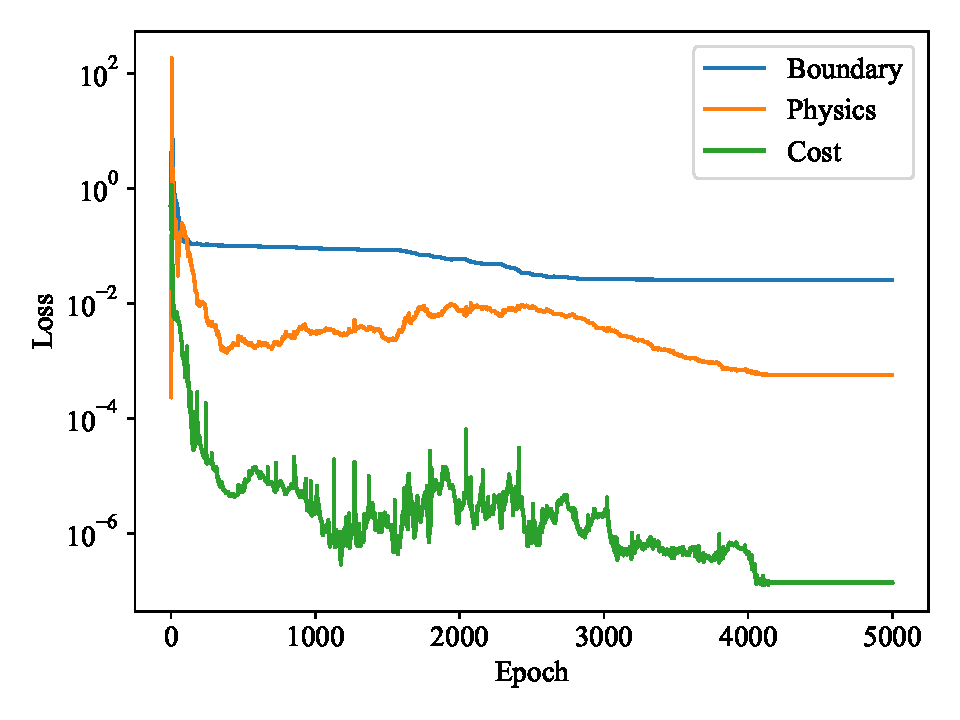
\includegraphics[width=1.0\linewidth]{Figures/IntermediateExperiments/OptimalControl/laplace_optimal_control_losses.pdf}
    \caption{Training losses when training for the optimal control problem on Laplace's equation.}
    \label{fig:laplace_optimal_control_losses}
\end{figure}

Another way to validate the learned control policy is to train a new PINN where the control policy is kept constant during training. For this experiment, this is equivalent to solving a standard boundary value problem. The objective function is not used for training, but is instead measured and used as a performance metric during training.

Doing this results in the output solution plot in Figure \ref{fig:laplace_optimal_control_validate} and losses in Figure \ref{fig:laplace_optimal_control_losses_validate}.

\begin{figure}[H]
    \centering
    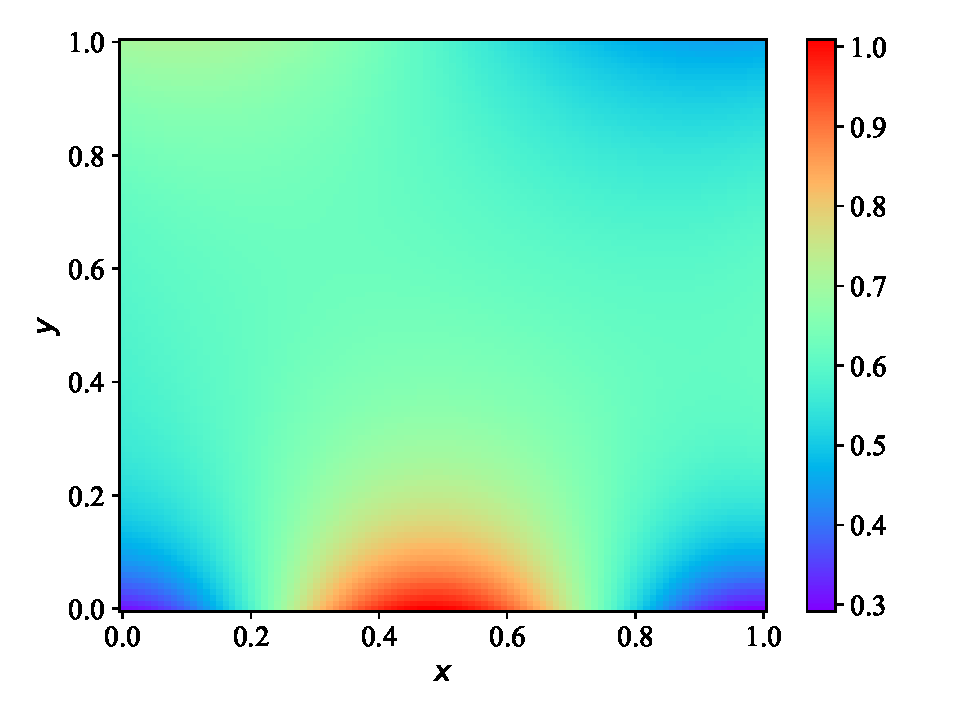
\includegraphics[width=1.0\linewidth]{Figures/IntermediateExperiments/OptimalControl/laplace_optimal_control_validate.pdf}
    \caption{Output solution to Laplace's equation with the control policy fixed as a boundary condition.}
    \label{fig:laplace_optimal_control_validate}
\end{figure}

The output plot looks relatively similar to the previous output plot, with the biggest differences around the boundary. However, by looking at the individual losses, the cost of the objective function is now significantly worse, which is an indication that the learned control policy would not work very well on a true system. The same problem remains with the fact that the learned control policy is not periodic, which can be why the physics loss is much lower than the boundary loss. But it is likely that it is not possible to find a solution that perfectly satisfies both the boundary conditions and the desired flux. A possible solution to the non-periodic control policy could be to satisfy the periodic boundary with a Fourier embedding in the y-direction, which could be worth investigating further.

\begin{figure}[H]
    \centering
    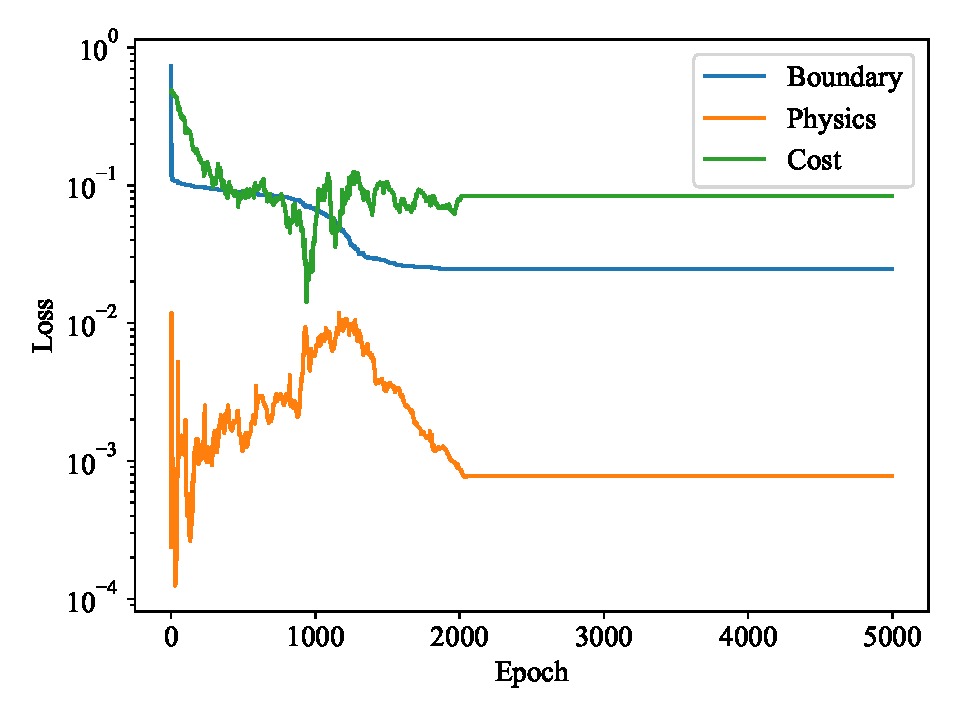
\includegraphics[width=1.0\linewidth]{Figures/IntermediateExperiments/OptimalControl/laplace_optimal_control_losses_validate.pdf}
    \caption{Training losses when training on Laplace's equation with the control policy fixed as a boundary condition. The cost is not used when training, and is instead used as a performance metric.}
    \label{fig:laplace_optimal_control_losses_validate}
\end{figure}

\subsubsection{Dirichlet Boundary Control}

Training a PINN on the output solution of the heat equation results in the plot shown below in Figure \ref{fig:heat1d_optimal_control_boundary2}, which looks relatively similar to the previous 1-dimensional heat equation plots. As the desired temperature distribution is a constant $0.5$, the system will attempt to move towards this distribution while also subject to the constraint of the dynamics. Figure \ref{fig:heat1d_optimal_control_boundary2_slices} shows the same plot viewed at some slices in time.

As seen from the time slices, the temperature distribution becomes flatter over time, but the heat equation is not really capable of staying constant over a bounded domain. It is possible that the temperature distribution would oscillate at the boundaries and remain close to 0.5 in the center, which overall averages out to 0.5 over a longer time horizon.

\begin{figure}[H]
    \centering
    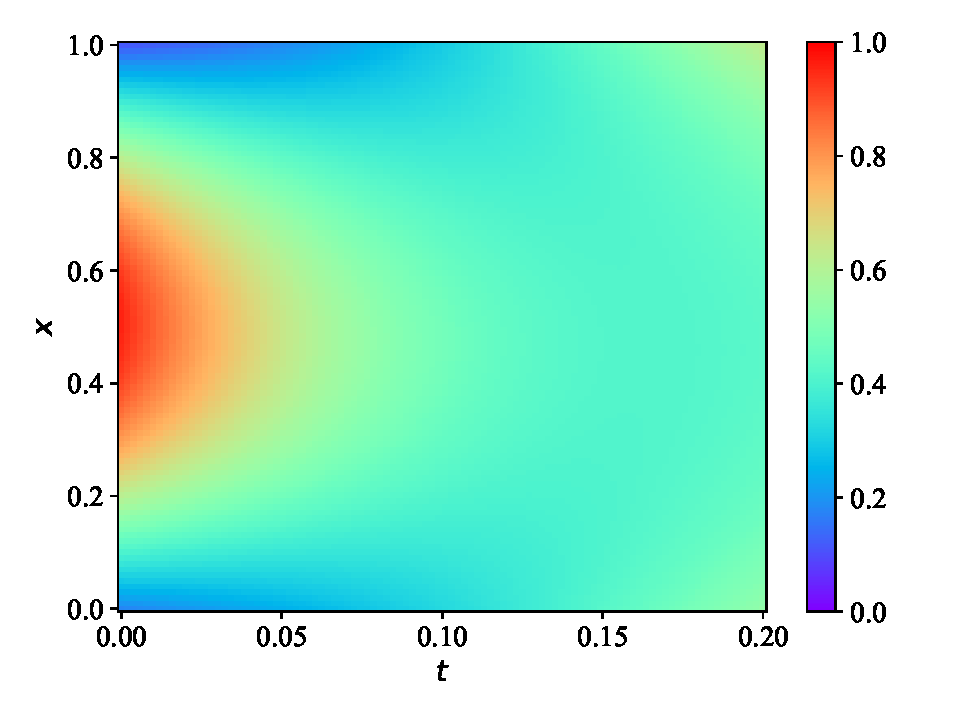
\includegraphics[width=1.0\linewidth]{Figures/IntermediateExperiments/OptimalControl/heat1d_optimal_control_boundary2.pdf}
    \caption{PINN output of the solution to the optimal control problem on the heat equation with Dirichlet boundary control.}
    \label{fig:heat1d_optimal_control_boundary2}
\end{figure}

\begin{figure}[H]
     \centering
     \begin{subfigure}[b]{0.5\textwidth}
         \centering
         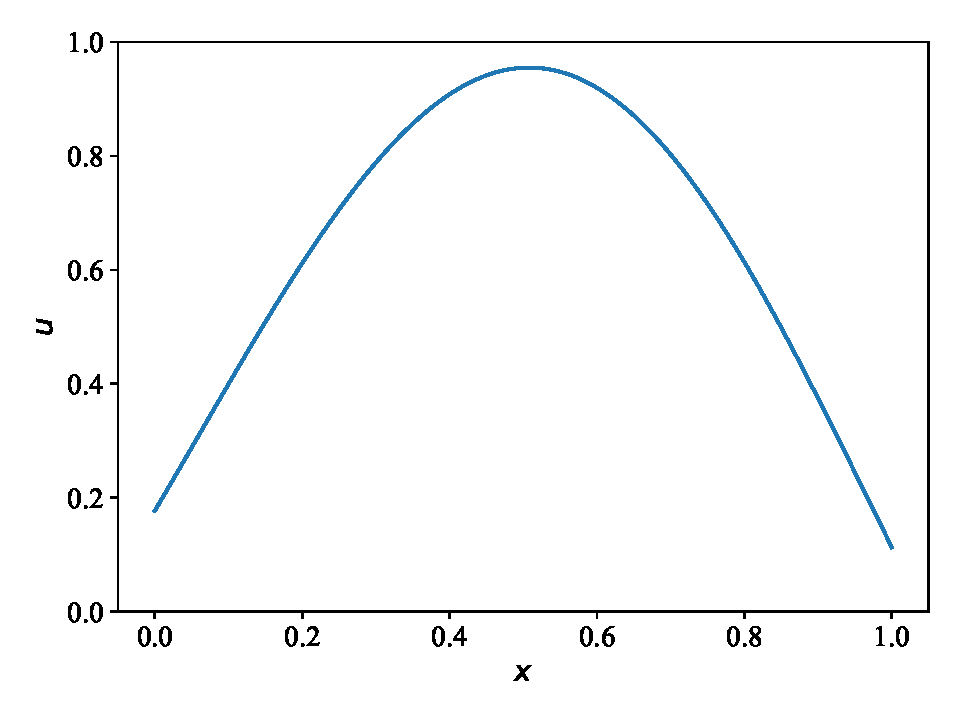
\includegraphics[width=\textwidth]{Figures/IntermediateExperiments/OptimalControl/heat1d_optimal_control_boundary2_slice1.pdf}
         \caption{$t = 0$}
         \label{fig:heat1d_optimal_control_boundary2_slice1}
     \end{subfigure}
     \vskip\baselineskip
     \begin{subfigure}[b]{0.5\textwidth}
         \centering
         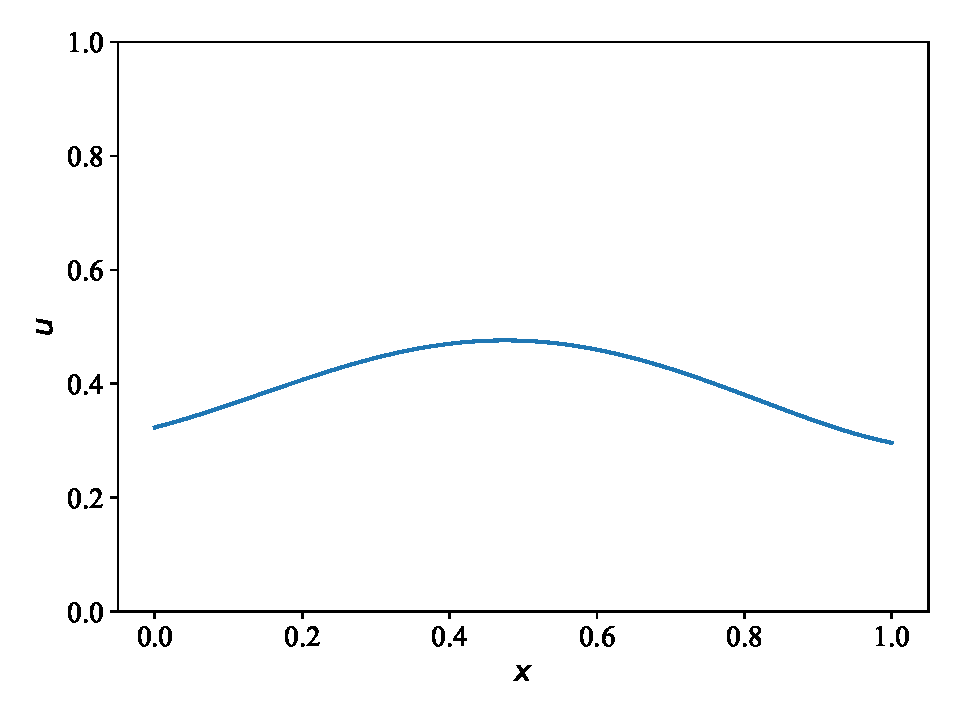
\includegraphics[width=\textwidth]{Figures/IntermediateExperiments/OptimalControl/heat1d_optimal_control_boundary2_slice2.pdf}
         \caption{$t = 0.1$}
         \label{fig:heat1d_optimal_control_boundary2_slice2}
     \end{subfigure}
     \vskip\baselineskip
     \begin{subfigure}[b]{0.5\textwidth}
         \centering
         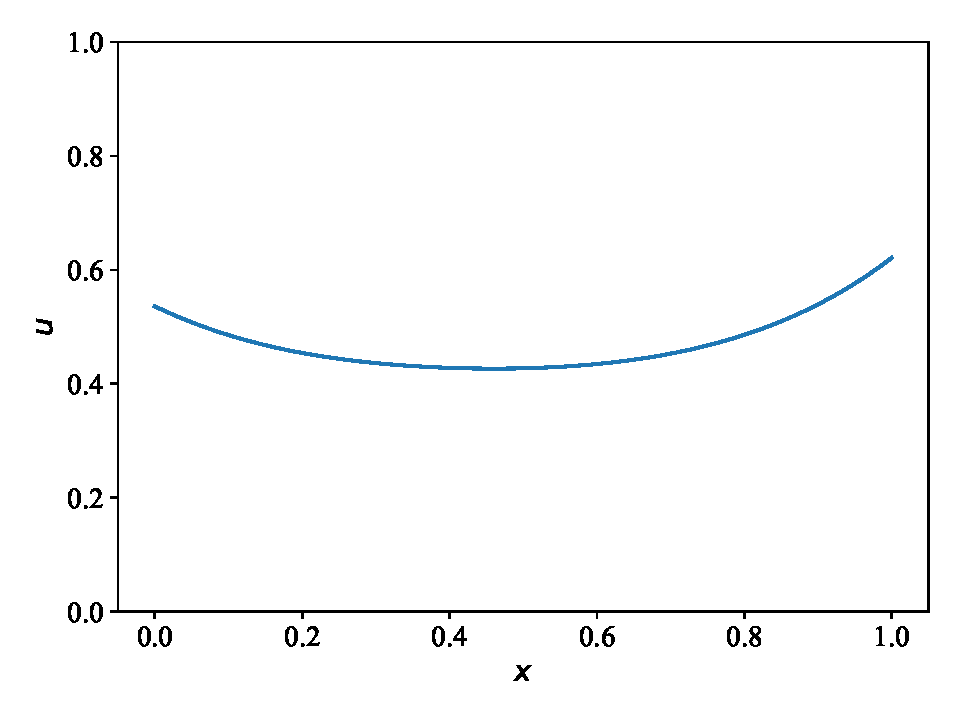
\includegraphics[width=\textwidth]{Figures/IntermediateExperiments/OptimalControl/heat1d_optimal_control_boundary2_slice3.pdf}
         \caption{$t = 0.2$}
         \label{fig:heat1d_optimal_control_boundary2_slice3}
     \end{subfigure}
    \caption{Visualization of time-slices from the PINN output of the solution to the optimal control problem on the heat equation with Dirichlet boundary control.}
    \label{fig:heat1d_optimal_control_boundary2_slices}
\end{figure}

\begin{figure}[H]
    \centering
    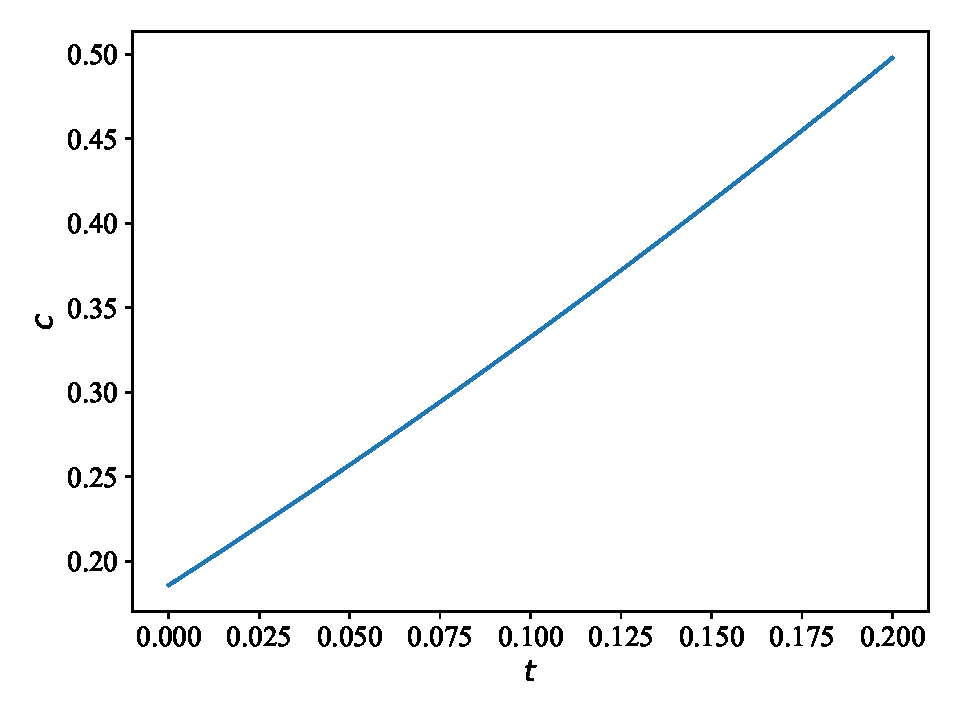
\includegraphics[width=1.0\linewidth]{Figures/IntermediateExperiments/OptimalControl/heat1d_optimal_control_boundary2_control.pdf}
    \caption{Learned control policy to the optimal control problem on the heat equation with Dirichlet boundary control.}
    \label{fig:heat1d_optimal_control_boundary2_control}
\end{figure}

The learned control policy is shown in Figure \ref{fig:heat1d_optimal_control_boundary2_control}, which also serves as a boundary condition along the bottom side of the domain. It appears as a linearly increasing function, which can make sense by considering that there is an initial heat distribution that is spread out over the domain over time. As the distribution becomes more spread out, there is also less incoming heat to the edges of the domain, which is compensated for by the control policy. This can also be justified by thinking of the heat equation as containing a first order partial derivative of time, which when integrated over time becomes a straight line.

As there is no boundary condition on the top, the trained PINN appears to impose a symmetric boundary condition on itself. This can be thought of as equivalent to applying the control boundary on both sides of the domain. For real systems governed by the heat equation on a bounded domain, there will always be some boundary conditions on both sides of the domain. This also means that real systems will typically get a more asymmetric distribution when supplied with heat from only one of the boundaries.

\subsubsection{Neumann Boundary Control}

Replacing the Dirichlet boundary with the Neumann boundary and training a PINN on the optimal control problem results in the output solution in Figure \ref{fig:heat1d_optimal_control_boundary1} along with time-slices in Figure \ref{fig:heat1d_optimal_control_boundary1_slices}. The desired temperature distribution is still set to be a constant 0.5.

\begin{figure}[H]
    \centering
    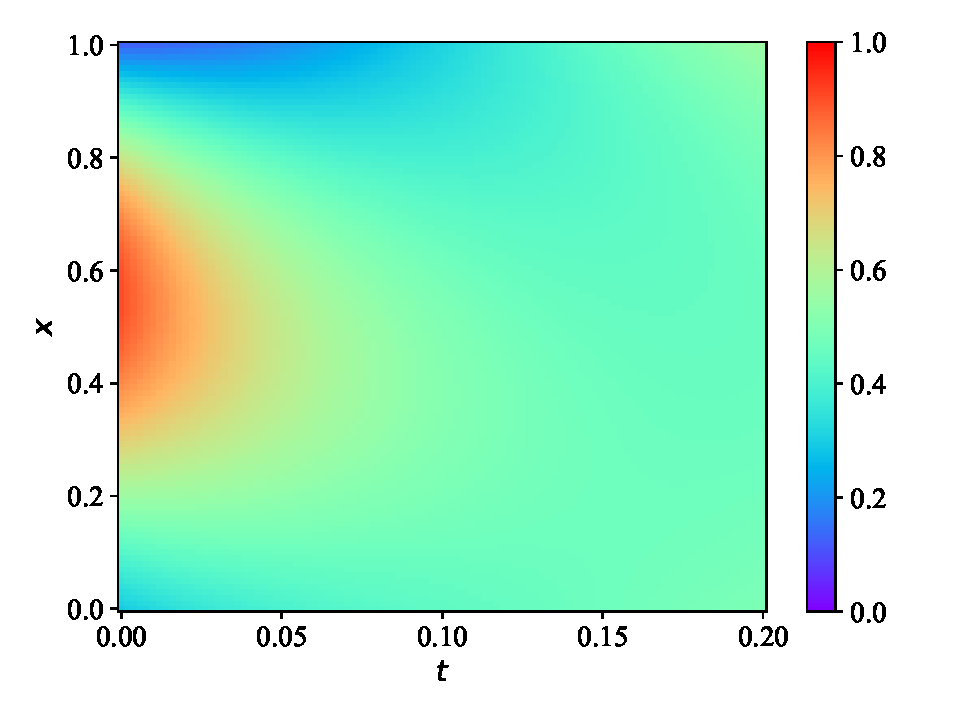
\includegraphics[width=1.0\linewidth]{Figures/IntermediateExperiments/OptimalControl/heat1d_optimal_control_boundary1.pdf}
    \caption{PINN output of the solution to the optimal control problem on the heat equation with Neumann boundary control.}
    \label{fig:heat1d_optimal_control_boundary1}
\end{figure}

One noticeable difference from the previous experiment is that the overall temperature distribution is much less symmetric. This also seems like a more realistic result, and might be related to how Neumann control can be interpreted as more realistic than Dirichlet control. Now, heat is sent in with some inertia, as opposed to instantly setting the heat on the boundary. Otherwise, the same heat distribution appears to flatten out relatively well, and the same argument related to averaging out over a longer time span is still valid.

\begin{figure}[H]
     \centering
     \begin{subfigure}[b]{0.5\textwidth}
         \centering
         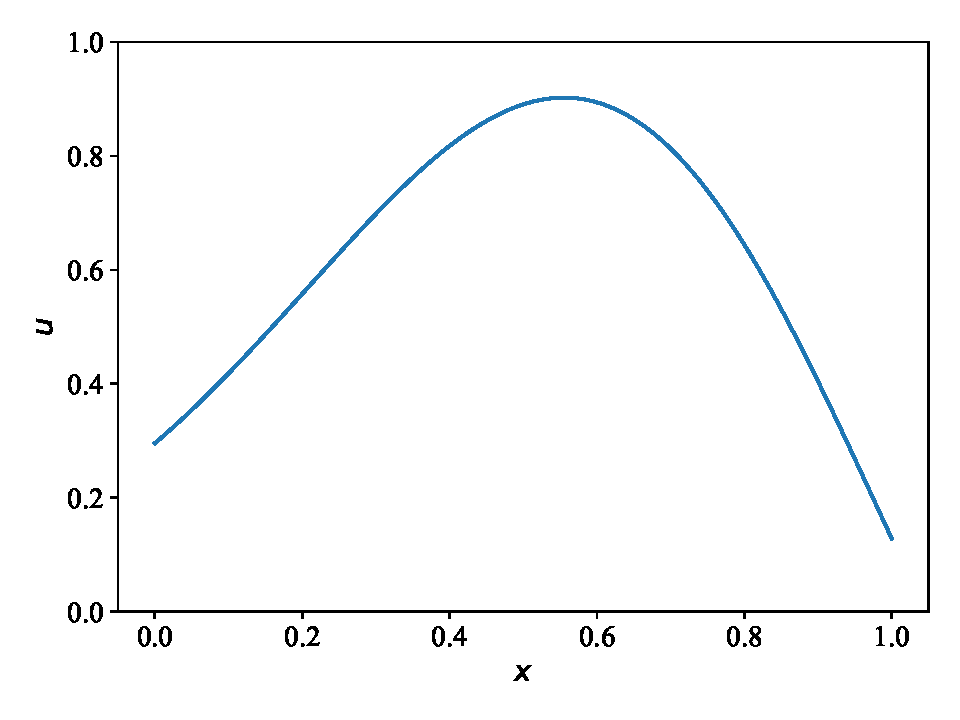
\includegraphics[width=\textwidth]{Figures/IntermediateExperiments/OptimalControl/heat1d_optimal_control_boundary1_slice1.pdf}
         \caption{$t = 0$}
         \label{fig:heat1d_optimal_control_boundary1_slice1}
     \end{subfigure}
     \vskip\baselineskip
     \begin{subfigure}[b]{0.5\textwidth}
         \centering
         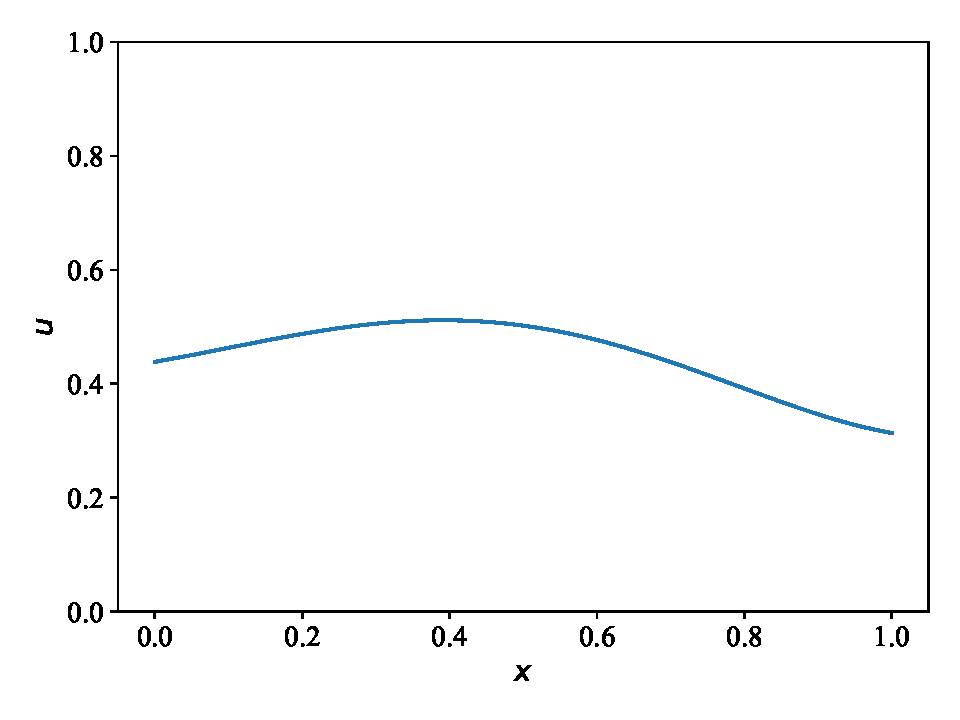
\includegraphics[width=\textwidth]{Figures/IntermediateExperiments/OptimalControl/heat1d_optimal_control_boundary1_slice2.pdf}
         \caption{$t = 0.1$}
         \label{fig:heat1d_optimal_control_boundary1_slice2}
     \end{subfigure}
     \vskip\baselineskip
     \begin{subfigure}[b]{0.5\textwidth}
         \centering
         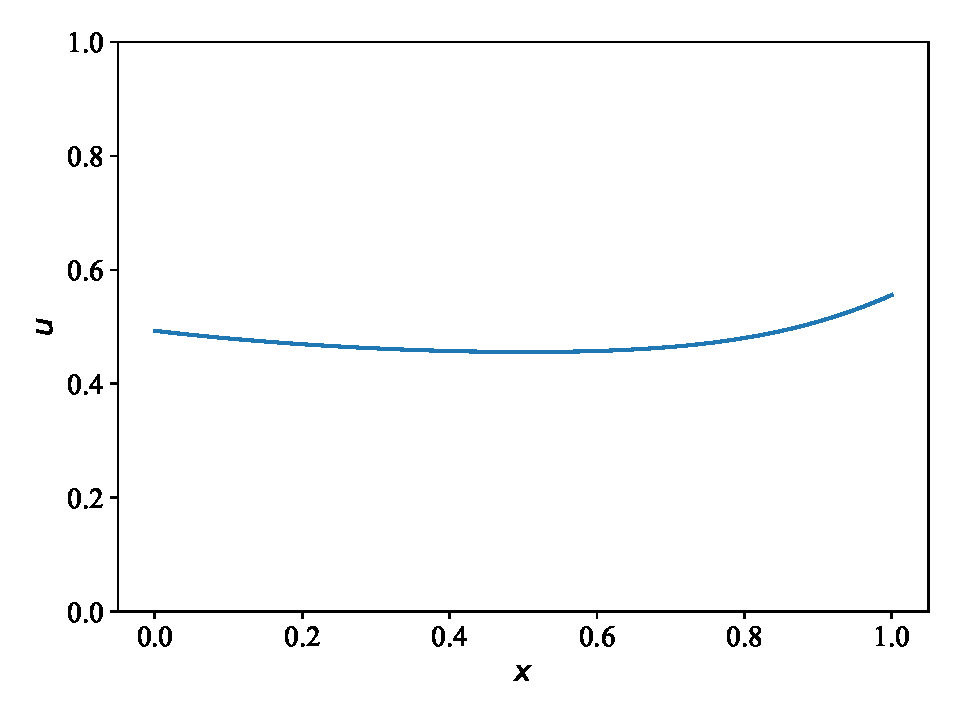
\includegraphics[width=\textwidth]{Figures/IntermediateExperiments/OptimalControl/heat1d_optimal_control_boundary1_slice3.pdf}
         \caption{$t = 0.2$}
         \label{fig:heat1d_optimal_control_boundary1_slice3}
     \end{subfigure}
    \caption{Visualization of time-slices from the PINN output of the solution to the optimal control problem on the heat equation with Neumann boundary control.}
    \label{fig:heat1d_optimal_control_boundary1_slices}
\end{figure}

\begin{figure}[H]
    \centering
    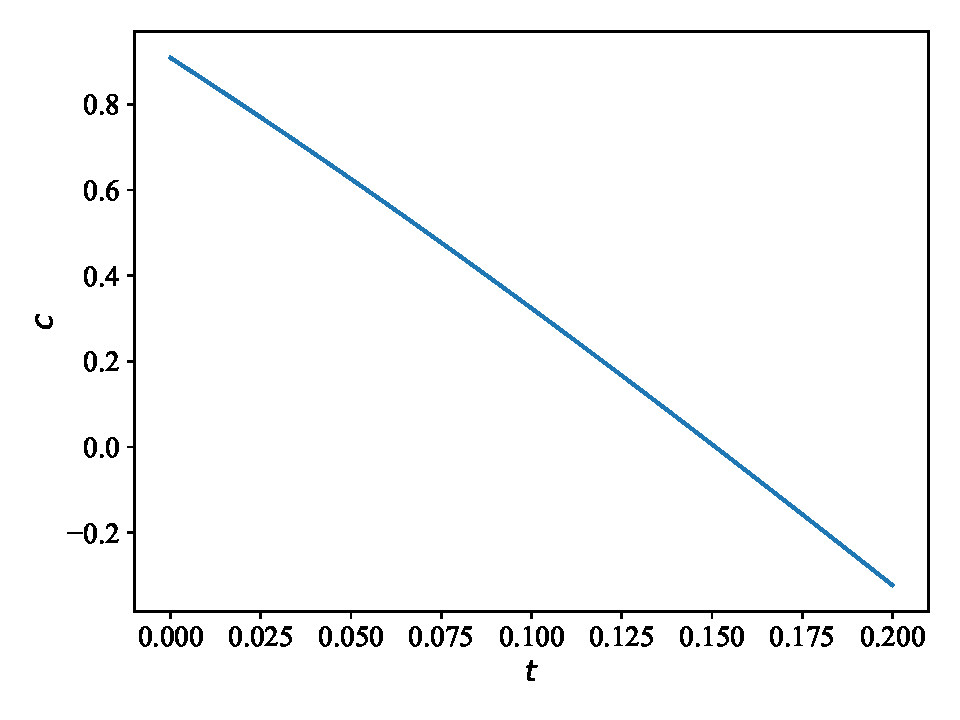
\includegraphics[width=1.0\linewidth]{Figures/IntermediateExperiments/OptimalControl/heat1d_optimal_control_boundary1_control.pdf}
    \caption{Learned control policy to the optimal control problem on the heat equation with Neumann boundary control.}
    \label{fig:heat1d_optimal_control_boundary1_control}
\end{figure}

The learned control policy in Figure \ref{fig:heat1d_optimal_control_boundary1_control} still appears as a straight line, although this time with a downward slope. As the value of $c(t)$ refers to the rate of change in the x-direction on the boundary, this is related to how much heat to introduce to the system. At the beginning the boundary is close to zero which means a high rate of heat must be introduced. After a while, as the heat distributes evenly, it is less necessary to add more heat. Eventually due to inertia, the heat on the boundary exceeds the desired heat of 0.5, so the rate of change becomes negative to lower it.

This overshoot might lead to some oscillations which could resemble a step response for an underdamped second order linear system, where it eventually approaches a stationary value. A reason for this could be because the objective function is set to target a heat distribution of a constant $0.5$ without considering the inertia in the heat distribution itself, causing it to overshoot on the boundaries. For the step response mentioned previously, the reference can be set to a constant value for the state, and a value of zero to the derivative of the state to account for this.

To test this hypothesis further, the same optimal control problem was solved again with a longer time horizon. The final time now goes from 0.2 to 1 second. The number of data points along the initial condition was also increased from 100 to 1000 to increase the general accuracy.

The resulting solution from this is plotted in Figure \ref{fig:heat1d_optimal_control_boundary1_longer} along with time slices in Figure \ref{fig:heat1d_optimal_control_boundary1_slices_longer}. The overall solution is now much more symmetric again, which could indicate that the previous lack of symmetry was more because of too few data points along the initial condition, thus making it asymmetric from the start. Because there still isn't any boundary condition on the top, it might be that the PINN imposes its own symmetry again.

\begin{figure}[H]
    \centering
    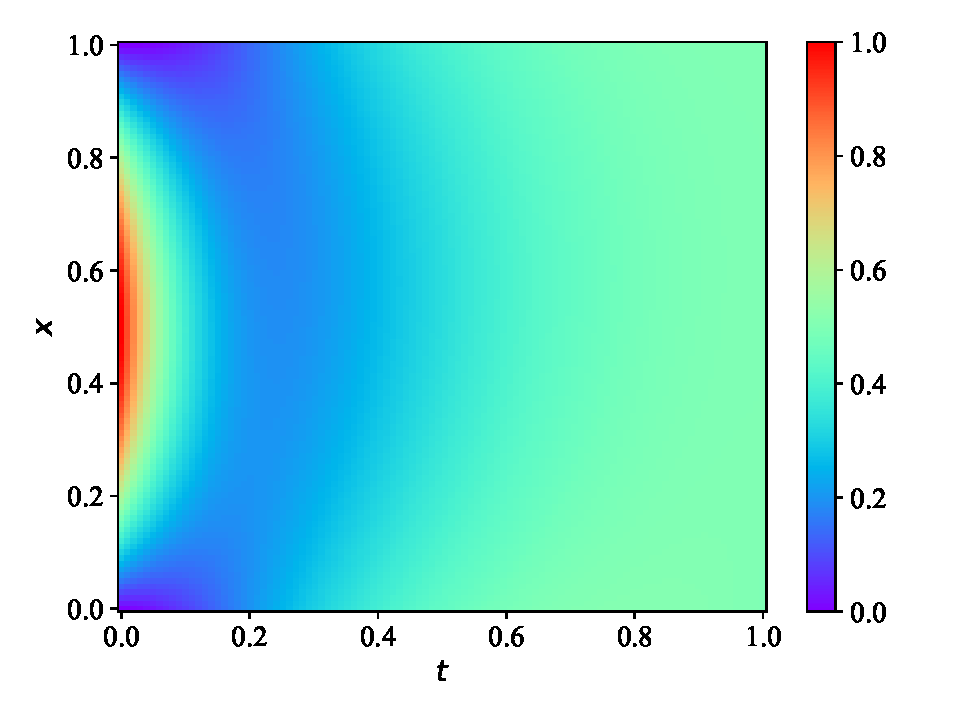
\includegraphics[width=1.0\linewidth]{Figures/IntermediateExperiments/OptimalControl/heat_neumann_longer/heat1d_optimal_control_boundary1.pdf}
    \caption{PINN output of the solution to the optimal control problem on the heat equation with Neumann boundary control and a longer time horizon.}
    \label{fig:heat1d_optimal_control_boundary1_longer}
\end{figure}

It is also interesting to note that the new plot in Figure \ref{fig:heat1d_optimal_control_boundary1_longer} appears to almost vanish completely in an arc a little after 0.2 seconds. As the desired temperature distribution is set to be at $t = 1$, it does not have to resemble the plot from the previous run. It is then brought back by the control input that gradually shapes the distribution.

\begin{figure}[H]
     \centering
     \begin{subfigure}[b]{0.5\textwidth}
         \centering
         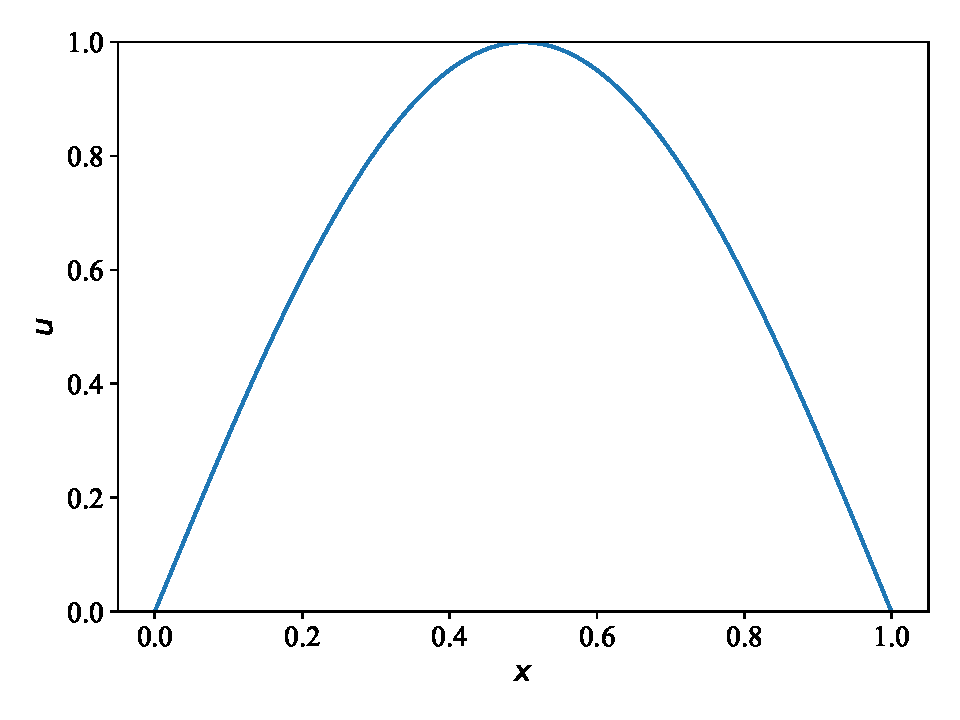
\includegraphics[width=\textwidth]{Figures/IntermediateExperiments/OptimalControl/heat_neumann_longer/heat1d_optimal_control_boundary1_slice1.pdf}
         \caption{$t = 0$}
         \label{fig:heat1d_optimal_control_boundary1_slice1_longer}
     \end{subfigure}
     \vskip\baselineskip
     \begin{subfigure}[b]{0.5\textwidth}
         \centering
         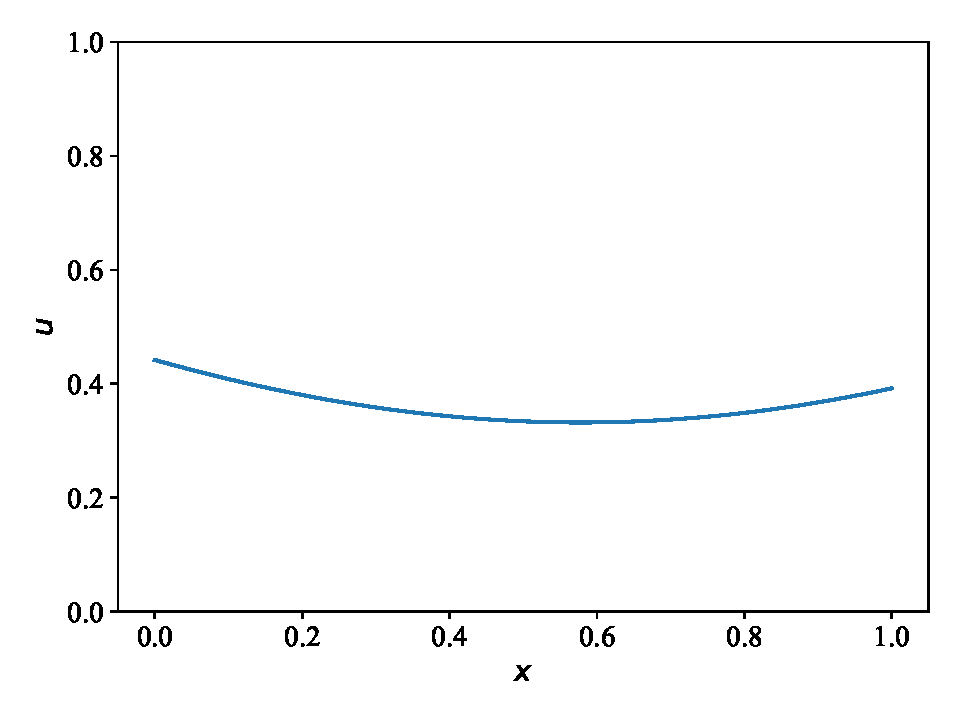
\includegraphics[width=\textwidth]{Figures/IntermediateExperiments/OptimalControl/heat_neumann_longer/heat1d_optimal_control_boundary1_slice2.pdf}
         \caption{$t = 0.1$}
         \label{fig:heat1d_optimal_control_boundary1_slice2_longer}
     \end{subfigure}
     \vskip\baselineskip
     \begin{subfigure}[b]{0.5\textwidth}
         \centering
         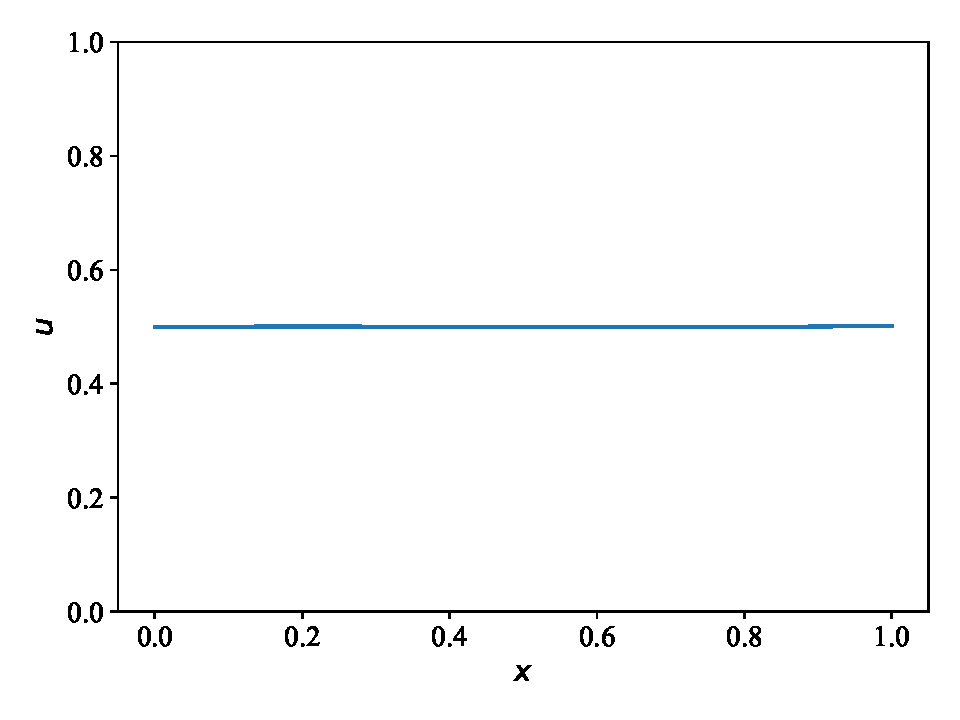
\includegraphics[width=\textwidth]{Figures/IntermediateExperiments/OptimalControl/heat_neumann_longer/heat1d_optimal_control_boundary1_slice3.pdf}
         \caption{$t = 0.2$}
         \label{fig:heat1d_optimal_control_boundary1_slice3_longer}
     \end{subfigure}
    \caption{Visualization of time-slices from the PINN output of the solution to the optimal control problem on the heat equation with Neumann boundary control and a longer time horizon.}
    \label{fig:heat1d_optimal_control_boundary1_slices_longer}
\end{figure}

\begin{figure}[H]
    \centering
    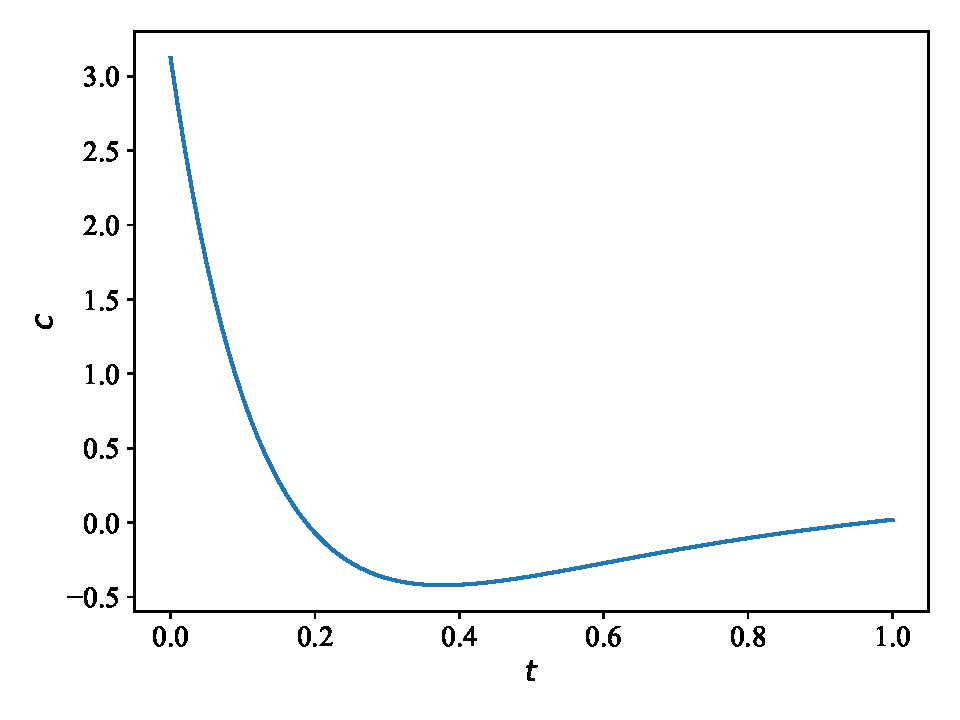
\includegraphics[width=1.0\linewidth]{Figures/IntermediateExperiments/OptimalControl/heat_neumann_longer/heat1d_optimal_control_boundary1_control.pdf}
    \caption{Learned control policy to the optimal control problem on the heat equation with Neumann boundary control and a longer time horizon.}
    \label{fig:heat1d_optimal_control_boundary1_control_longer}
\end{figure}

The control input visualized in Figure \ref{fig:heat1d_optimal_control_boundary1_control_longer} looks similar to the previous input in the sense that it looks like a relatively straight line at the start. It also overshoots zero, before slowly converging back to it from below, which is very reminiscent of a second order step response that is slightly underdamped. At the end with a time derivative of zero, it means that the rate of change in the x direction is zero. Which shows that the heat distribution has converged to a constant value.

\subsubsection{Initial Control}

For the final optimal control experiment, the trained PINN output is visualized in Figure \ref{fig:burger_control}. Comparing the plot visually to the analytical plot, it is immediately clear that it is not a good representation of the true solution. Looking at specific slices in time shown in Figure \ref{fig:burger_control_slices}, the differences become more obvious. The learned solution at the initial time $t = 0$ also corresponds to the learned control policy, and does match the analytical solution very well. However, the PINN appears to still converge to the desired analytical solution at $t = 5$ to a high degree, which also corresponds to satisfying the objective function well.

\begin{figure}[H]
    \centering
    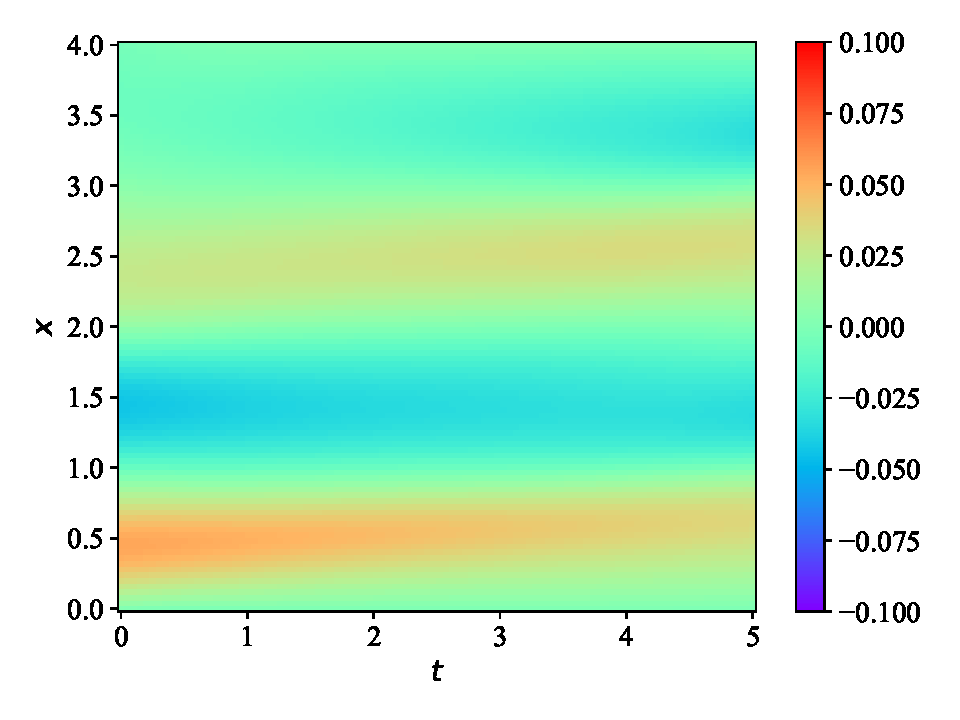
\includegraphics[width=1.0\linewidth]{Figures/IntermediateExperiments/OptimalControl/burger_control.pdf}
    \caption{PINN output of the solution to the optimal control problem with Burgers' equation.}
    \label{fig:burger_control}
\end{figure}

\begin{figure}[H]
     \centering
     \begin{subfigure}[b]{0.45\textwidth}
         \centering
         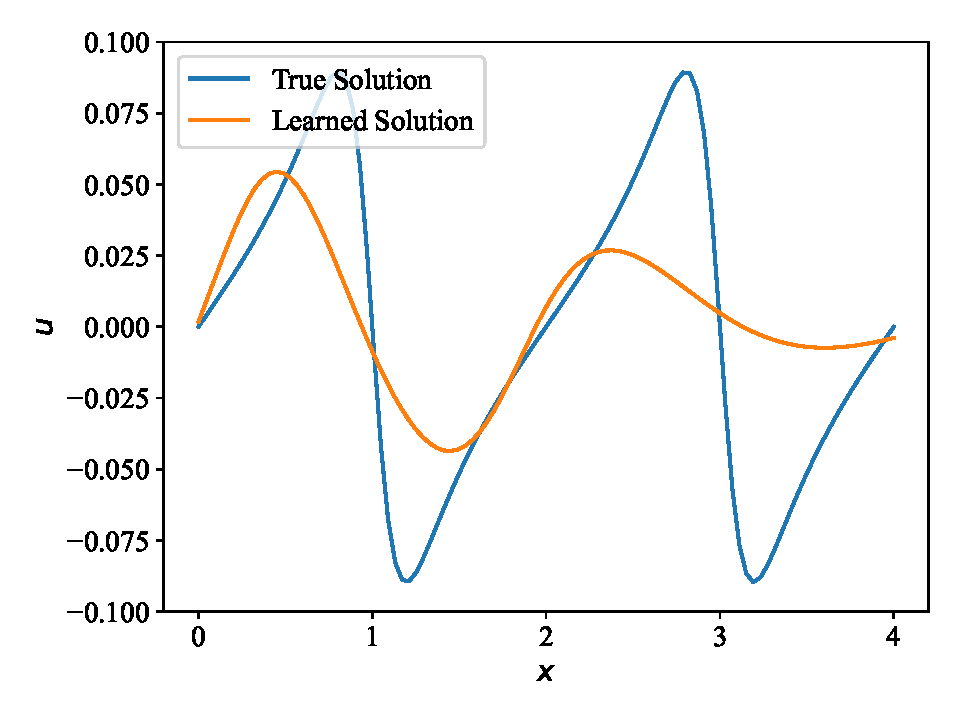
\includegraphics[width=\textwidth]{Figures/IntermediateExperiments/OptimalControl/burger_control_slice0.pdf}
         \caption{$t = 0$}
         \label{fig:burger_control_slice0}
     \end{subfigure}
     \hfill
     \begin{subfigure}[b]{0.45\textwidth}
         \centering
         \includegraphics[width=\textwidth]{Figures/IntermediateExperiments/OptimalControl/burger_control_slice1.pdf}
         \caption{$t = 5$}
         \label{fig:burger_control_slice1}
     \end{subfigure}
    \caption{PINN output at specific slices in time of the solution to the optimal control problem with Burgers' equation.}
    \label{fig:burger_control_slices}
\end{figure}

Looking at the individual training losses in Figure \ref{fig:burger_control_losses}, it can be seen that the boundary loss is the lowest, which means that the network is not obstructed in the same way as previous experiments. The initial loss comes next, and refers to the difference between the control policy and initial value. So even with a low initial loss, the large discrepancy comes because the control policy itself is inaccurate. The cost of the objective function comes next, leaving the physics informed loss as the worst performing. So this can indicate that even though the learned control policy worked well to lower the objective function here, it would not work well when applied to a real system, as the physics cheat to get there.

\begin{figure}[H]
    \centering
    \includegraphics[width=1.0\linewidth]{Figures/IntermediateExperiments/OptimalControl/burger_control_losses.pdf}
    \caption{Training losses when training for the optimal control problem with Burgers' equation.}
    \label{fig:burger_control_losses}
\end{figure}

The plots in Figure \ref{fig:burger_control_losses} are generally noisy with many frequent spikes. The spikes happen at the same times when the Adam optimizer is stuck in a local minima but is carried outside with momentum. Then the physics loss increases somewhat, while the other three increase. This essentially means that it is a difficult problem to solve with this simple formulation. The plots also appear to converge at the end. This happens because of a change to the L-BFGS optimizer at 18000 epochs. But it also looks like the L-BFGS optimizer simply converges to the same local minima the models already were bouncing around in with Adam, and might not be necessary to use.

\subsection{Regularization with the Maximum Principle}

\subsubsection{Elliptic PDE}

Regularizing the training by using the maximum principle for Laplace's equation results in the PINN output in Figure \ref{fig:laplace_trained}, which overall looks very similar to the analytical solution in Figure \ref{fig:laplace_analytical}. Calculating the MSE from the analytical solution results in $1.21 \cdot 10^{-4}$. For comparison, training another PINN from scratch with the exact same setup except the regularization results in an MSE from the analytical solution of $1.91 \cdot 10^{-4}$. So the regularization yields a very small improvement.

\begin{figure}[H]
    \centering
    \includegraphics[width=1.0\linewidth]{Figures/IntermediateExperiments/Laplace/laplace_forward.pdf}
    \caption{PINN output after training with maximum principle regularization on Laplace's equation.}
    \label{fig:laplace_trained}
\end{figure}

Plotting this MSE value as a validation loss for each epoch when training results in the plots in Figure \ref{fig:laplace_losses}. The regularized PINN appears to learn faster during the first 200 epochs before flattening out. It then eventually surpasses the standard PINN again after around 700 epochs.

It is possible that the regularization is something that works best at the start of training, and can then be gradually or completely removed from the loss function. But it does seem to give slightly faster training along with a little better final performance / accuracy. And as the computational cost is insignificant in comparison to the rest of the training, adding this regularization term when training on elliptic PDEs does not seem to have any obvious disadvantages. However, while the performance gains are very minor for this specific experiment, it could be more useful for elliptic PDEs in higher dimensions, and might be interesting to investigate further.

\begin{figure}[H]
    \centering
    \includegraphics[width=1.0\linewidth]{Figures/IntermediateExperiments/Laplace/maxmin_losses.pdf}
    \caption{Validation losses after training with maximum principle regularization on Laplace's equation.}
    \label{fig:laplace_losses}
\end{figure}

\subsection{Causal Optimal Control}

\subsubsection{Initial Control}

Training a PINN with causal training and the other mentioned improvements results in the plots shown below in Figure \ref{fig:burger_control_initial_attempt1} and Figure \ref{fig:burger_control_initial_slices_attempt1}.

\begin{figure}[H]
    \centering
    \includegraphics[width=1.0\linewidth]{Figures/AdvancedExperiments/InitialControlCausal/attempt1/burger.pdf}
    \caption{PINN output of the solution to the optimal control problem with Burgers' equation after training with causality and other improvements.}
    \label{fig:burger_control_initial_attempt1}
\end{figure}

\begin{figure}[H]
     \centering
     \begin{subfigure}[b]{0.45\textwidth}
         \centering
         \includegraphics[width=\textwidth]{Figures/AdvancedExperiments/InitialControlCausal/attempt1/burger_slice0.pdf}
         \caption{$t = 0$}
         \label{fig:burger_control_initial_slice0_attempt1}
     \end{subfigure}
     \hfill
     \begin{subfigure}[b]{0.45\textwidth}
         \centering
         \includegraphics[width=\textwidth]{Figures/AdvancedExperiments/InitialControlCausal/attempt1/burger_slice1.pdf}
         \caption{$t = 5$}
         \label{fig:burger_control_initial_slice1_attempt1}
     \end{subfigure}
    \caption{PINN output at specific slices in time of the solution to the optimal control problem with Burgers' equation after training with causality and other improvements.}
    \label{fig:burger_control_initial_slices_attempt1}
\end{figure}

Comparing these results visually to the previous attempt in Figure \ref{fig:burger_control} and Figure \ref{fig:burger_control_slices} it is overall a better result, which is easier to see when $t = 0$. It is also possible that further training would give even better results, as the causality makes the overall training take much longer for a problem like this. Another consideration is that the relative weighting of the physics loss is set to a really large value, which is necessary to not be overrun by the causal loss and initial loss.

However, the initial condition is still not very good when compared with the analytical solution. It is possible that the causality makes the problem too difficult to learn. Running the same experiment again with the same setup with all the improved techniques except for the causal loss results in the Figures shown below in Figure \ref{fig:burger_control_initial_attempt3} and Figure \ref{fig:burger_control_initial_slices_attempt3}.

\begin{figure}[H]
    \centering
    \includegraphics[width=1.0\linewidth]{Figures/AdvancedExperiments/InitialControlCausal/attempt3/burger.pdf}
    \caption{PINN output of the solution to the optimal control problem with Burgers' equation after training with many improvements, but not causality.}
    \label{fig:burger_control_initial_attempt3}
\end{figure}

\begin{figure}[H]
     \centering
     \begin{subfigure}[b]{0.45\textwidth}
         \centering
         \includegraphics[width=1.0\linewidth]{Figures/AdvancedExperiments/InitialControlCausal/attempt3/burger_slice0.pdf}
         \caption{$t = 0$}
         \label{fig:burger_control_initial_slice0_attempt3}
     \end{subfigure}
     \hfill
     \begin{subfigure}[b]{0.45\textwidth}
         \centering
         \includegraphics[width=1.0\linewidth]{Figures/AdvancedExperiments/InitialControlCausal/attempt3/burger_slice1.pdf}
         \caption{$t = 5$}
         \label{fig:burger_control_initial_slice1_attempt3}
     \end{subfigure}
    \caption{PINN output at specific slices in time of the solution to the optimal control problem with Burgers' equation after training with causality and other improvements.}
    \label{fig:burger_control_initial_slices_attempt3}
\end{figure}

The solution looks relatively similar to the previous attempt that used causality. The initial condition is the biggest change, where the amplitude is closer to the true solution but some of the skewness is lost. It is hard to say which attempt resulted in the best solution, and that might depend on what the application of the problem would be.

\subsubsection{Reversed Initial Control}

Using the time-reversed PDE and training a PINN on these dynamics while also using causality and the other training techniques described before results in Figure \ref{fig:burger_control_initial_reversed} and Figure \ref{fig:burger_control_initial_slices_reversed}.

\begin{figure}[H]
    \centering
    \includegraphics[width=1.0\linewidth]{Figures/AdvancedExperiments/InitialControlCausal/reversed/burger.pdf}
    \caption{PINN output of the solution to the optimal control problem with Burgers' equation after training on the time-reversed system.}
    \label{fig:burger_control_initial_reversed}
\end{figure}

\begin{figure}[H]
     \centering
     \begin{subfigure}[b]{0.45\textwidth}
         \centering
         \includegraphics[width=1.0\linewidth]{Figures/AdvancedExperiments/InitialControlCausal/reversed/burger_slice0.pdf}
         \caption{$t = 0$}
         \label{fig:burger_control_initial_slice0_reversed}
     \end{subfigure}
     \hfill
     \begin{subfigure}[b]{0.45\textwidth}
         \centering
         \includegraphics[width=1.0\linewidth]{Figures/AdvancedExperiments/InitialControlCausal/reversed/burger_slice1.pdf}
         \caption{$t = 5$}
         \label{fig:burger_control_initial_slice1_reversed}
     \end{subfigure}
    \caption{PINN output at specific slices in time of the solution to the optimal control problem with Burgers' equation after training on the time-reversed system.}
    \label{fig:burger_control_initial_slices_reversed}
\end{figure}

These final results from training on the time-reversed dynamics can be seen to improve upon the previous attempts by looking at the initial learned solution. While still not perfect, it is a noticeable improvement from the ones in Figure \ref{fig:burger_control_initial_attempt1} and Figure \ref{fig:burger_control_initial_attempt3}. This plot was here generated by sampling at the final time for the trained model to get the initial distribution to use. Using this problem formulation, training with causality also makes more sense as it is working in the same way as the dependence between final state and initial condition.

This experiment shows the importance of adapting the method to the problem. Not all problems become easier by time-reversing the dynamics, but in cases like this where it is possible it resulted in a solution that was easier to learn.

%\section{Lessons Learnt}
%Discuss about the weaknesses of your work and explain how you will do things differently given a chance to repeat the full study.

\section{Discussion}

% Rewrite this section after the results are done

Modeling dynamical systems with standard neural networks is often difficult due to a lack of training data, and the trained networks struggle with generalization outside the training domain. Adding prior physics information about the dynamics, which can often be obtained by modeling systems from first principles, can regularize the neural networks in a way that both allows them to learn from much less data and also generalize much better outside the domain of the training data.

A non-intuitive result was that complicated dynamics turned out to be easier to learn compared to more difficult dynamics, the exact opposite of what usually happens when working with dynamical systems. As complicated dynamical systems are more strict in how the system evolves it is possible that they also contain more information when training PINNs, which allows for easier training. In general, it appears that PDEs are easier to learn than ODEs, time-varying is easier than time-invariant, and nonlinear is easier than linear.

How the training is done can also greatly influence the final result. Using the correct optimization algorithm turned out to be important for some problems. Having enough collocation points is necessary for better generalization, and is also necessary for increasing the number of training steps. The collocation points should also be placed at the correct locations. A linearly spaced grid makes learning very difficult, while a random uniform sampling often works well enough. 

Discovering unknown system parameters is one of the main advantages of PINNs compared to traditional numerical methods, and seems to work well for simple problems. This does however require significantly more training data, and is also much more computationally expensive. Learning terms symbolically has the problem where the input variables must be explicitly set. This could mean that to find the best overall solution it requires that the PINN is trained from scratch from every possible input combination if nothing prior is known. And without access to an analytical solution or data it is not possible to verify the solution, which is always the case when using the method for new problems.

Using PINNs for optimal control problems are possible to setup, and the framework has shown to be very flexible and easy to setup for solving many different types of problems, requiring a relatively low complexity for the implementation. The results are however very difficult to accurately verify, and the method does not have any convergence guarantees. This stands in contrast to traditional numerical optimization methods, where a convex optimization problem has algorithms that provably converge to the global optimum. Of course not all problems are convex, but many of practical interest are possible to formulate like this.